\chapter{Trajectory Planning}
\label{chapter:trajectory_planning}

The main focus of this thesis is the problem of trajectory planning for a fast moving car. In this chapter, we will analyze this problem in depth. We will first look into the planning problem in general and then we will discuss what the term ``fast moving cars'' means and how trajectory planning for a fast car is different from the general planing problem.

With the knowledge of the theory, we will formulate our trajectory planning problem. We will consider several well-known search algorithms used to solve planning problems and adapt them to our problem.

The solution of the planning problem will be a trajectory. A trajectory is the description of both the path the vehicle should follow and the speed profile. If a robot is able to follow this trajectory, it will have an advantage over reactive steering algorithms, such as end-to-end driving, as it will be able to go through a series of corners efficiently by slowing down and accelerating at convenient times and by following an appropriate racing line. We will discuss a way of following the trajectory later in Chapter~\ref{chapter:following}.

\section{Introduction to Planning}

In this section, we will give a brief overview of the basic concepts of automatic planning and planning under differential constraints. The main source of the information for this chapter is a book by Steven M. LaValle called \textit{Planning Algorithms} \cite{lavalle_2006}. This book describes all of the topics in this section in much more detail and it is a good source of further information on this topic.

\subsection{Automatic Planning}

Planning is the task of solving a problem by finding a sequence of actions, which transforms the world to some desired state. The world of a planning problem is defined in terms of states and actions.

A single state is a full description of all of the important aspects of the world. A state can be encoded in many different ways, for example it can be a set of logical propositions which hold true in the given state or a vector of an $n$-dimensional vector of real numbers. All of the possible states of the world form a state space.

An action is a way of changing a state of the world into a different state. Not all actions can be applied in all states and so the set of possible actions can differ from state to state. All of the actions together then form an action space.

The planning task is to find a sequence of actions, which changes the state of the world from a given initial state to some desired state. Such sequence of actions is referred to as a feasible plan.

With the intuition of what a planning problem is, we can formulate it formally:

\begin{defn}[Planning Problem]
	\label{def:basic_planning_problem}
	A planning problem is a tuple $\left(X, U, f, x_0, g\right)$ consisting of:
	
	\begin{enumerate}
		\item A \textit{nonempty set} $X$ of world states, called the \textit{state space}.
		\item For each state $x\in X$, a set of actions $U(x)$.  A set of all actions $U=\bigcup\limits_{x\in X} U(x)$ is called an \textit{action space}.
		\item A \textit{state transition function} $f$ defined for every $x\in X$ and $u\in U(x)$, which produces the state of the world after applying the action $u$ to the state $x$.
		\item An \textit{initial state} of the world $x_0\in X$.
		\item A goal region $X_g\subset X$.
	\end{enumerate}
\end{defn}

\begin{defn}[Feasible Plan]
	A solution to a planning problem $\left(X, U, f, x_0, g\right)$ is a \textit{feasible plan}, which a finite sequence of actions $\langle u_0, u_1, \ldots, u_k\rangle\in U^*$ such that:	
	\begin{gather*}
		\forall i \in \left\{0,1,\ldots,k\right\}: u_i\in U(x_i) \wedge x_{i+1}=f(x_i, u_i) \\
		x_{k+1} \in X_g.
	\end{gather*}
\end{defn}

\begin{defn}[Optimal Plan]
	Let $\left(X, U, f, x_0, g\right)$ be a planning problem and $\Pi=\left\{\pi\in U^* \mid \pi \text{ is a feasible plan}\right\}$ a set of all feasible plans. We say that a plan $\pi^*\in \Pi$ is an optimal plan with respect to a cost function $\gamma: \Pi \rightarrow \mathbb{R}$ if
	
	\[
		\pi^*=\argmin_{\pi\in\Pi} \gamma(\pi).
	\]
\end{defn}

\subsubsection{Reachability Graph}

We can imagine that the states form vertices of a graph $G=(V, E)$ and the applications of actions through the state transition function form directed edges between the vertices:

\begin{equation*}
\begin{aligned}
	V&=X \\
	E&=\left\{(x_1, x_2) \mid \exists u \in U(x_1): x_2 = f(x_1, u) \right\}.
\end{aligned}
\end{equation*}

This graph can in general have several subgraphs. We are only interested in the component, which contains the initial $x_0$ and all the vertices which are reachable from $x_0$ via a directed path. A feasible plan is then a directed path in the graph starting in the initial state vertex $x_0$ and ending in any of the goal states vertices. Finding a path in a graph is well-studied problem and there are several efficient algorithms to solve it, such as the Dijkstra algorithm or its extension called A*.

The size of the state space and the action spaces has great impact on the way how we approach the planning problem and how we find a solution. If the graph is finite or if the the number of vertices is countably infinite and the branching factor is finite, we can find the solution (if one exists) with a systematic search algorithm in a finite amount of time. If no solution exists and the graph is infinite, the algorithm will be trying different plans infinitely. In practice this can be avoided with a limiting criterion, such as maximum length of a plan.

When the number of vertices is uncountably infinite or the branching factor is infinite, the problem becomes much harder and we cannot rely on a simple graph search anymore. We will soon see that the state space of all of the vehicle configurations in our problem is uncountably infinite. These problems can be solved using \textit{sampling algorithms}.

We must keep in mind that the number of states of the system can be very high even if it is finite because the state space represents all of the combinations of the state variables of the world.

\subsection{Planning Under Differential Constraints}
\label{sec:planning_under_differential_constraints}

When describing the motion of a car-like robot on a two-dimensional plane, we assume that we can treat it as a rigid body, usually represented as a bounding rectangle. The configuration of the rigid body is then described by the pose of the vehicle: the $\left(x,y\right)$ Cartesian coordinates of a fixed reference point of the body in the world reference frame, and the heading angle $\theta$ between the longitudinal axis of the vehicle and the $x$ axis of the world reference frame. The $(x, y)$ location is in some bounded area $P\subset\mathbb{R}^2$ and the heading angle is an arbitrary angle $\theta\in\left[0,2\pi\right)$. This simple configuration space already has three continuous dimensions and it is uncountably infinite.

The kinematics and dynamics of robots are typically described by differential equations. These equations give us the velocities at which the state of the robot changes when an action is applied. As an example of these constraints, we can look at a model of a \textit{simple car} \cite[Section~13.1.2.1]{lavalle_2006}.

\begin{example}
The state space of a simple car will consist of the poses in an infinite 2D plane $(x, y, \theta)$ as described earlier. The control inputs are two dimensional vectors $\left(u_s, u_\varphi\right)$, where $u_s$ is the commanded speed of the vehicle in the direction perpendicular to the rear axis, and $u_\varphi$ is the steering angle of the front wheels. For a better understanding of this example, see the Figure~\ref{fig:simple_car}.

For a car with a wheelbase length $L\in\mathbb{R}$, the velocity can be approximated by this set of equations:

\begin{equation}
\begin{aligned}
	\dot{x}&=u_s \cos \theta \\
	\dot{y}&=u_s \sin \theta \\
	\dot{\theta}&=\dfrac{u_s}{L} \tan u_\varphi.
\end{aligned}
\end{equation}
\end{example}

\begin{figure}
	\centering
	
	\begin{tikzpicture}[
	axis/.style={thin, densely dashed, gray},
	axle/.style={thick, gray},
	vec/.style={ultra thick, ->, >=latex}
	]
	
	% the axes
	\path[name path=AX] (-1,0)--(8,0);
	\draw[thick, ->] (-1,0)--(8,0) node[right]{$x$};
	\draw[thick, ->] (0,-1)--(0,6.5) node[above]{$y$};
	
	\def\stateTheta{45} % heading angle of the vehicle
	\def\statePhi{-24} % steering angle of the front wheels
	\def\L{2.5} % wheelbase of the vehicle
	\def\W{1.45} % axle width
	\def\w{2} % width of the vehicle
	\def\l{4.5} % length of the vehicle
	\def\wW{0.2} % wheel width
	\def\wL{0.5} % wheel length
	\def\xoffset{3cm}
	\def\yoffset{0.8cm}
	
	% the rotated vehicle
	\begin{scope}[xshift=\xoffset, yshift=\yoffset]
	\begin{scope}[rotate=\stateTheta]
    
   		% longitudinal axis
   		\path[name path=AL] (-2.5, \w/2) -- (\l+2, \w/2);
   		\draw[axis] (-2.5, \w/2) -- (\l+2, \w/2);

		% visualize theta
		\path [name intersections={of=AL and AX, by={X}}];
		\draw[rotate=-\stateTheta] (X)++(0.7,0) arc (0:\stateTheta:0.7) node[right, yshift=-1mm, xshift=1mm] {$\theta$}; % theta
    
    	% shape of the vehicle
		\draw (0, 0) rectangle (\l, \w);		
		
		% axle coordinates
		\def\rearX{\l/2 - \L/2}
		\def\frontX{\l/2 + \L/2}
		\def\rightY{\w/2 - \W/2}
		\def\leftY{\w/2 + \W/2}
		
		\coordinate (front) at (\frontX, \w/2);
		\coordinate (rearLeft) at (\rearX, \w/2 + \W/2);
		\coordinate (frontLeft) at (\frontX, \w/2 + \W/2);
		
		% visualize the wheelbase length		
		\draw[axis] (rearLeft) -- ++(0, 1);
		\draw[axis] (frontLeft) -- ++(0, 1);		
		\draw[<->, >=latex] ($ (rearLeft) + (0, 0.8) $) -- node[above, xshift=-1.5mm, yshift=-1mm] {$L$} ($ (frontLeft) + (0, 0.8) $);
		
		\filldraw[axle] (\rearX, \rightY + \wW/2) -- (\rearX, \leftY - \wW/2); % the axle 
		\draw[thick] (\rearX - \wL/2, \rightY - \wW/2) rectangle (\rearX + \wL/2, \rightY + \wW/2); % rear right wheel/tire
		\draw[thick] (\rearX - \wL/2, \leftY - \wW/2) rectangle (\rearX + \wL/2, \leftY + \wW/2); % rear left wheel/tire
		
		% front axle
		\draw[thick, rotate around={\statePhi:(\frontX, \rightY)}] (\frontX - \wL/2, \rightY - \wW/2) rectangle (\frontX + \wL/2, \rightY + \wW/2); % rear right wheel/tire
		\draw[thick, rotate around={\statePhi:(\frontX, \leftY)}] (\frontX - \wL/2, \leftY - \wW/2) rectangle (\frontX + \wL/2, \leftY + \wW/2); % rear left wheel/tire
		\filldraw[axle] (\frontX, \rightY + \wW/2) -- (\frontX, \leftY - \wW/2); % the axle 
		
		% connect the axles
		\draw[axle] (front) -- (\rearX, \w/2);
		
		% xy
		\filldraw[] (\rearX, \w/2) circle (2pt) node[right, xshift=1mm] {$(x, y)$};
		
		% visualize phi
		\draw[axis, rotate around={\statePhi:(front)}] (front) -- (\frontX + 2, \w/2);
		\draw (front)++(0.7,0) arc (0:\statePhi:0.7) node[right, yshift=-2mm] {$\varphi$}; % theta
		
	
    \end{scope}
	\end{scope}
	
	\end{tikzpicture}
		
	\caption{The simple car from the example has three state variables. The speed and the steering angle are action variables and they can change at any moment, so the vehicle can stop on a spot and change the steering angle instantaneously, which is of course not possible in a real world car.}
	\label{fig:simple_car}
\end{figure}

The configuration space of all possible transformations of the robot and possibly additional variables required to keep the state of the kinematics and dynamics of the robot together form a continuous \textit{state space} $X$. In the example of the simple car, the state space would be just the configuration space itself, therefore $X=\mathbb{R}^2\times\left[0,2\pi\right)$, but different models could have more dimensions as we will see in Section~\ref{sec:vehicle_model}.

\paragraph{Obstacles}

Additionally, we must be able to split the state space $X$ into two complementary subsets: the obstacle region $X_{obs}\subseteq X$ and the free region $X_{free}=X\setminus X_{obs}$. Only the states in $X_{free}$ can be entered safely while the states in $X_{obs}$ must be avoided to prevent collisions of the robot with obstacles.

\paragraph{State Transition Function}

In order to be able formulate the planning problem for a system with differential constraints, we must change the meaning of the \textit{state transition function} $f$ from the previous Definition~\ref{def:basic_planning_problem}. This function used to produce the next state $x'$ after an action $u$ is applied to a state $x$, i.e. $x'=f(x, u)$. When the state space is continuous, the outcome of an execution of an action depends on for how long it is being applied. Instead of a direct transition to the next state, the function $f$ will now express the velocity in the state space as defined by the differential constraints:

\[
	\dot{x}=f(x, u).
\]

The function $f$ must be defined for every $x\in X$ and $u\in U(x)$. The task of a planning algorithm is then to find an \textit{action trajectory} which produces a collision-free \textit{state trajectory} which reaches a goal state. An \textit{action trajectory} is a continuous function $\tilde{u}: T \rightarrow U\cup\left\{u_t\right\}$ which maps an infinite interval $T=\left[0, \infty\right)$ to an action, which should be executed at the given point in time. From a point in time $t_{end}\in\left[0, \infty\right)$, a termination action $u_t$ can be applied to mark the end of the action trajectory ($\forall t>t_{end}: \tilde{u}(t)=u_t$). To \textit{state trajectory} corresponding to the action trajectory $\tilde{u}$ is a function $\tilde{x}: T \rightarrow X$, such that $\tilde{x}(0)$ is a given initial state $x_0$, and $\forall t \in \left(0, t_{end}\right]$:

\begin{equation}
	\label{eq:integrate_state_trajectory}
	\tilde{x}(t) = \tilde{x}(0) + \int_0^t f(\tilde{x}(\tau), \tilde{u}(\tau)) d\tau,
\end{equation}

such that $\forall \tau\in\left[0, t_{end}\right]: \tilde{u}(\tau)\in U(\tilde{x}(\tau))$. A collision-free trajectory adds a requirement to go only through the free region ($\tilde{x}(\tau)\in X_{free}$).

\begin{defn}[Planning Problem Under Differential Constraints]
	\label{def:planning_problem_under_differential_constraints}
	A planning problem under differential constraints $\left(X, U, f, x_0, g\right)$ is an extension planning problem given in Definition~\ref{def:basic_planning_problem}, such that:
	
	\begin{enumerate}
		\item The state space $X$ is continuous.
		\item A \textit{state transition function} $f$ defined for every $x\in X$ and $u\in U(x)$, which produces the velocity in the state space after applying the action $u$ to the state $x$: $\dot{x}=f(x, u)$.
	\end{enumerate}
\end{defn}

\begin{defn}[Feasible Plan]
	A solution to a planning problem under differential constraints $\left(X, U, f, x_0, g\right)$ is a \textit{feasible action trajectory} $\tilde{u}$ when $\exists t_{end} \in \left(0, \infty\right)$ such that:
	\begin{gather*}
	\forall t \leq t_{end}: \tilde{u}(t)\in U(\tilde{x}(t)) \\
	\tilde{x}(t) = \tilde{x}(0) + \int_0^t f(\tilde{x}(\tau), \tilde{u}(\tau)) d\tau \\
	\tilde{x}(t_{end})\in X_g.
	\end{gather*}
\end{defn}

\subsubsection{Sampling-Based Planning Methods}

In order to be able to plan in a world with a continuous state space and continuous time, sampling-based methods can be used. The main idea is to discretize the action trajectory by using the same action for a non-trivial time period. This effectively discretizes time into time intervals, which usually have a fixed length $\Delta t$ or the duration depends on the action which is used (``a motion primitive'' \cite[Section~14.2.3]{lavalle_2006}). The action trajectory can then be expressed as a simple sequence of actions and for every action in the sequence it is possible to determine the time at which it is supposed to be applied and for how long it is supposed to be applied. We can still obtain a continuous trajectory through the state space by integrating the action sequence.

Ideally, every segment of a state trajectory obtained by integrating an action from a state over a time period should be checked for collision. In practice, this could be very resource intensive, and so only a few samples (sometimes only the end state of the segment) are tested using a ``black box'' collision detection function to see if the segment is in $X_{obs}$ or $X_{free}$.

If the action space is infinite, it should be sampled as well and only a finite number of actions should be considered. This makes it possible to construct a graph where samples of $X$ are the vertices and the edges between them are actions. Starting from $x_0$, we compute all of the possible state trajectories starting in this state with all the actions in the finite set of actions over a time period (either a fixed $\Delta t$ or a time associated with the action) and add the final states as vertices to the graph and connect them with directed edges to the origin state. We repeat this for all added states over and over again.

The size of the graph is affected also by the discretization of time. The shorter the time interval is, the larger the graph will be. Nevertheless, we can perform graph search over and find solutions to planning problems with differential constraints. We will describe concrete search algorithms for our problem in Section~\ref{sec:trajectory_planning_algorithms}.

The discretization of time might make some states of the state space unreachable and this could make finding a feasible plan impossible. In order to achieve resolution-completeness of the sampling based algorithm, every time a plan is not found, the discretization should be made finer (e.g., by decreasing the length of the time intervals by half) \cite[Chapter~14.2]{lavalle_2006}.

\section{Trajectory Planning For Fast Moving Cars}

In this section we will discuss what it means to plan a trajectory for a fast moving car. What is the difference between trajectory planning for a slow moving car and for a fast moving car? What do we even consider to be a ``fast moving car'' and what is just a slow moving car?

\subsection{Terminology Clarification}

A fast moving car is not a widely used term and it does not have a formal definition. Intuitively, we would consider a ``fast moving car'' to be a Formula 1, a rally car, or a different racing car. The racing drivers push their vehicles to their limits in order to be the first one behind the finish line. We might also consider ordinary driving on a motorway to be ``fast'', especially during a lane change maneuver or when we accelerate to overtake a vehicle in front of us. We might even consider driving at lower speeds to be ``fast'' when it involves taking sharp turns.

One thing these scenarios have in common is that the car reaches a speed at which it can become hard to steer the car in a specific direction because the tires might lose grip and the car might start moving sideways or in a more extreme scenario the car could roll over sideways. The speed which could be considered ``fast'' varies based on the radius of the turn.

For the purposes of this thesis, we will formulate the term in the following definitions:

\begin{defn}[Handling limits of a vehicle]
	We say, that a car is moving at its handling limits during a turn of a radius of $r\in(r_{min}, \infty]$ meters, if it is driving close to a speed $v_{max,r}$ at which the total force vector acting on the body of the vehicle would exceed the forces of the tires which keep the vehicle traveling at the constant radius $r$.
\end{defn}

The minimum turning radius $r_{min}\in\mathbb{R}$ is a constant specific for a given vehicle. It refers to the minimum turning radius which the vehicle can achieve at a very low speed and with the maximum steering angle possible. We can consider driving straight as driving along a circle with the radius of $\infty$ meters.

\begin{defn}[Fast moving car]\label{def:fast_moving_car}
	A car is moving fast when it is approaching its handling limits during a turn.
\end{defn}

\begin{defn}[Trajectory planning problem for a fast moving car]
	We say that a trajectory planning problem for a fast moving car is a planning problem under differential constraints. The solution of this problem is a collision-free time-optimal state trajectory and the vehicle does not at any point in time exceed its handling limits. The \textit{state trajectory} is describes both a path and a speed profile for the given vehicle and track.
\end{defn}


To achieve a time-optimal trajectory, we will search for a trade off between the length of the path and the speed at any given moment. To keep within the handling limits of the vehicle, our differential constraints must closely model the behavior of the vehicle. Even if our model of the vehicle describes its behavior well, it is more than likely that the robot will deviate from the planned trajectory at some point. The noise in sensor readings, imperfections in the actuators, or imprecise map of the track, all of these factors will contribute to errors in trajectory tracking. At some point, the difference between the planned path and velocity profile of the vehicle will be so large, that it will be advantageous to create a new plan from the current pose and speed of the vehicle. To make this possible, we need to be able to re-plan the trajectory in a short period of time.

Given our assumption, that we will most likely have to re-plan the trajectory at some point in the future anyway, it does not make too much sense to plan the trajectory for the whole circuit at once. The longer the trajectory we are planning, the longer it will take to find a suitable plan. Instead, we could split the track into multiple shorter segments and plan a trajectory only for a few of the segments directly in front of the current pose of the vehicle.

When the vehicle is moving fast, a belated or too early decision to change the direction or adjust the speed of the vehicle might result in a crash or a sub-optimal trajectory. Fast reaction times are therefore key. If we plan a trajectory for only a limited stretch in front of the vehicle, we must be able to find the plan for the following stretch before we reach the end of the current reference trajectory. Failing to do this, the vehicle will not have a trajectory to follow and it would probably have to preform some kind of an emergency braking in order to prevent collisions, or it would be forced to resort to some simpler reactive steering strategy, which does not involve planning ahead and which would most likely be sub-optimal.

We can now summarize the discussion in this section into a set of requirements for the trajectory planning algorithm which will make it more suitable for fast moving cars:

\begin{itemize}
	\item The whole track should be split into smaller segments, so that we do not have to waste resources to plan a trajectory for segments which will most likely not be reached by the time we will need to re-plan the trajectory.
	\item The differential constraints of the vehicle must accurately describe the movement of the vehicle at its handling limits and we must be able to eliminate dangerous maneuvers, which could lead to a crash or a trajectory or which could not be followed closely by the vehicle.
	\item The search algorithm we will use must find good solutions which are time-optimal or close to time-optimal in a very short period of time.
\end{itemize}

\subsection{Problem Analysis}

\subsubsection{The Configuration Space and the State Space}
\label{sec:configuration_and_state_space}

We only consider the motion of our vehicle on a two-dimensional flat surface. For simplicity, we will consider the shape of the vehicle to be a rectangle of a constant width and height, which fully encloses all of the parts of the body of the vehicle. This gives us a simple way of checking collisions with obstacles and by adjusting the size of the rectangle we can also add a small safety margin around the vehicle to stay on the ``safe side'' when closely passing obstacles.

Any position of the boundary rectangle in the 2D plane can be expressed as a rigid body transformation. We will define a \textit{configuration space} $C$ consisting of all these possible transformations of the vehicle. Each transformation can be expressed as a vector $\left( x, y, \theta\right)\in \mathbb{R}^2\times \left[0, 2\pi\right)$ where $\left( x, y\right)$ are the coordinates of the center of gravity of the vehicle (corresponding to the center of the rectangle) and $\theta$ is the angle between the $x$ axis of the coordinate system and the longitudinal axis of the vehicle, i.e. the heading angle of the vehicle.  This configuration space is continuous.

The complete \textit{state space} $X$ of the vehicle will be a combination of the configuration space $C$ and additional variables representing the kinematics and dynamics required by the differential constraints. We will define a function $\kappa: X\rightarrow C$ which returns the configuration of the vehicle in the given state, and also $\kappa_{x,y}: X\rightarrow \mathbb{R}^2$ and $\kappa_\theta: X\rightarrow \left[0, 2\pi\right)$ to obtain just the position or the heading angle of the given state. We will discuss the choice of appropriate vehicle models in Section~\ref{sec:vehicle_model} and we will define a concrete state space for each of the vehicle models.

\paragraph{Initial State}
At the start of the race, the vehicle is expected to be situated at a predefined starting location of the racing circuit with its heading angle identical to the direction of the race. The vehicle starts from a standstill with the wheels not spinning and the front wheels pointing the heading direction of the car.

During the race, the speed and the steering angle have to be measured using sensors. We must take into account that this state is most likely slightly inaccurate due to the errors in the measurements and due to a delay between the measurement and the start of planning. By the time the planning algorithm finds a trajectory, the state vehicle will have already changed and it will be different from the initial conditions of the planning algorithm.

\subsubsection{Collision Detection}

A collision detection function $c_{R}: C \rightarrow \left\{T, F\right\}$ divides the configuration space into two parts $C_{free}$ and $C_{obs}$:

\begin{equation*}
\begin{aligned}
	C_{obs} &= \left\{x\in C \mid c_{R}(x)=T\right\} \\
	C_{free} &= C \setminus C_{obs}.
\end{aligned}
\end{equation*}

The subscript $R$ represents a specific instance of the collision detection function for a rectangular shape of a specific width and height. The task of the collision detection function is to determine if the boundary rectangle of the vehicle in the given configuration $x\in C$ collides with some obstacle in the world or not. This function is the only way how the planning algorithm can determine the shape of the track and any additional obstacles which appear on the track.

The planning algorithm does not work directly with the configuration space, but rather with a state space. An extension of the partitioning into $C_{free}$ and $C_{obs}$ into the state space is very straightforward because a collision is dependent only on the configuration of the vehicle body, not on the kinematics and dynamics of the vehicle. For a state $x\in X$, which is an extension a configuration $c_x \in C$, it holds $x\in X_{obs} \iff c_x\in C_{obs} \wedge x\in X_{free} \iff c_x\in C_{free}$.

\paragraph{Representation of Obstacles}
We represent the obstacles in the world as an occupancy grid. An \textit{occupancy grid} is a matrix $O_r^{m\times n}\in \left\{0, 1\right\}^{m\times n}$ where $m,n\in\mathbb{N}$ is the size of the grid and $r\in\mathbb{R}$ is the resolution. Every element of the matrix represents a square tile of $r\times r$ meters placed in a grid covering an area of $rm\times rn$ square meters. The tiles can be in two states: either it can be traversed freely, or there is some obstacle in the tile and so the tile must be avoided. This is represented by the values $0$ (free space) and $1$ (an obstacle) in our definition.

To check if a single point of the world $\left(x,y\right)\in \mathbb{R}^2$ collides with an obstacle or not, we must first determine the coordinates of the tile in which it belongs:

\begin{equation*}
\begin{aligned}
	x_r &= \left\lceil \frac{x}{r} \right\rceil \\
	y_r &= \left\lceil \frac{y}{r} \right\rceil
\end{aligned}
\end{equation*}

If the point lies outside of the area covered by the occupancy grid, we can treat it as an obstacle. Otherwise we look into the appropriate cell of the matrix. The collision detection function $c_1$ for a single point can be:

\begin{equation*}
	c_1(O_{r}^{m\times n}, x, y) =
	\begin{cases}
		1 & x_r < 1 \lor y_r < 1 \lor y_r > m \lor x_r > n \\
		\left(O_{r}^{m\times n}\right)_{y_r, x_r} & \text{otherwise}.
	\end{cases}
\end{equation*}

We assume that the occupancy grid is aligned with the origin of the world reference frame and that the column indexes grow parallel to the $x$ axis and the indexes of rows parallel to the $y$ axis. If there is a transformation between the origin of the world reference frame and the occupancy grid, the point $(x, y)$ has to be rotated and translated appropriately before the coordinates of the corresponding tile can be determined. Please note that matrix rows and columns are indexed from 1, unlike for example arrays in the C and many other programming languages, which start indexing at 0.

We chose the occupancy grid because it is a standard way of representing 2D maps in \gls{ROS}, especially when a robot is equipped with a \gls{LIDAR}. We used these technologies to build our custom experimental vehicle and therefore we also used this map representation.

\paragraph{Moving Obstacles}
In this thesis, we will not consider moving obstacles. If it was necessary, we would have to extend the definition of the collision detection function to include a time parameter and it would have to extrapolate and predict a state of the world at the given time and check the collision against this prediction. The rest of the planning algorithm would not be affected by this extension.

\paragraph{Collision Detection Implementation}
The collision detection function must be evaluated every time the planning algorithm considers a use of an action from some state. If the action would lead to a state which would collide with an obstacle, this action should not even be allowed. The complexity of the collision detection function will therefore have a great impact on the performance of the algorithm on real hardware.

The footprint of the body of the vehicle is a rotated rectangle and we have to check if any of the parts of this rectangle does not hit an obstacle cell. We considered two versions of the collision detection algorithm:
\begin{enumerate}
	\item Pre-calculating small occupancy grids for several configurations of the vehicle and overlaying them with the occupancy grid representing the world.
	\item Inflating the obstacles in the occupancy grid and performing a single point check.
\end{enumerate}

The idea of \textit{the first method} is to calculate a list of tiles relative to the tile in which the center of the rectangle lies which the vehicle could collide with. We would split the heading angle dimension of the configuration into several regular intervals. For each of these intervals we would take the value in the middle and use it as a heading angle $\theta$. We would then rotate the bounding rectangle by the angle $\theta$ and mark which cells of a grid with the resolution $r$ it would overlay. We must take into consideration that the center of the rectangle can be at any point of the tile and different cells would be overlaid for example when the center coincides with the top left corner of the cell or the bottom right corner. Figure~\ref{fig:collision_detection_overlap} depicts this idea. To check collisions, we would first determine the cell corresponding to the center of the bounding rectangle of the vehicle and determine the discretization of the heading angle $\theta$. For the discretized heading angle, we would then remember a list of integer coordinates of the cells which would be occupied relative to the center of the rectangle. We would then check the state of the occupancy grid for the tiles occupied by the footprint of the vehicle and if any of them was marked as $X$ or if the coordinate would be outside of the bounds of the $m\times n$ grid, we would report a collision.

\begin{figure}[!tbp]%
	\centering
	\begin{subfigure}[t]{0.45\textwidth}
		\centering
		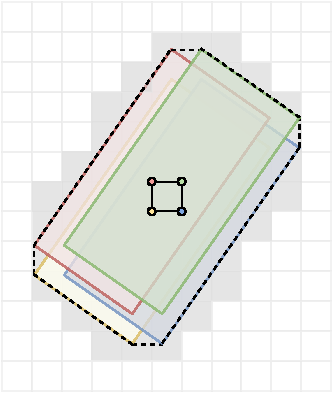
\includegraphics[width=0.95\textwidth]{../img/footprint}
		\caption{The figure shows which tiles can be occupied by the vehicle when the heading angle is close to $\theta$ for a center anywhere in the cell which contains its center. The dashed line is a boundary of all possible configurations of the vehicle. The dark gray squares are the grid cells which should be tested for collision.}
		\label{fig:collision_detection_overlap}
	\end{subfigure}
	\hfill
	\begin{subfigure}[t]{0.45\textwidth}
		\centering
		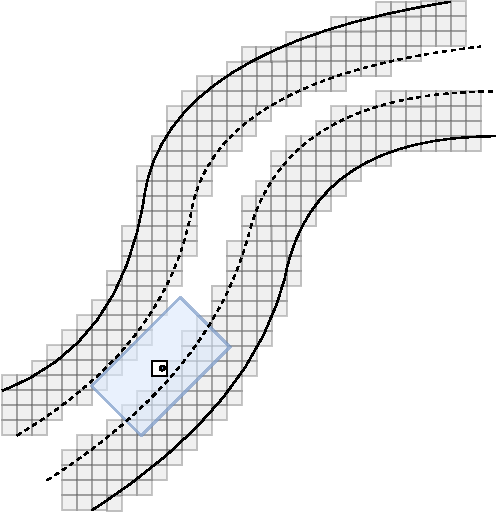
\includegraphics[width=0.95\textwidth]{../img/obstacle_inflation}
		\caption{The obstacles are ``inflated'' by the radius of the vehicle and every cell, which is closer to any obstacle than the radius of the vehicle is marked as dangerous. To detect collision, it is necessary to check if the cell which contains the center of the vehicle body is dangerous or not.}
		\label{fig:collision_detection_inflation}
	\end{subfigure}
	
	\caption{These figures compare two approaches to collision checking. The second approach requires fewer operations whenever we need to test a collision and therefore we chose the ``obstacle inflation'' method.}
\end{figure}

\textit{The second idea} is simpler. First, we determine the minimum safe distance of the vehicle from the width and length of the vehicle. We will then change all free tiles in the occupancy grid to obstacle tiles if they are closer to an original obstacle tile than the minimum radius and ``inflate'' the obstacles. To check for collisions of a vehicle at position $(x, y)$, only a single invocation of $c_1$ is required which has very little performance requirements. This method is depicted in Figure~\ref{fig:collision_detection_inflation}.

The obvious advantage of the first method is its higher accuracy. The second method could be insufficient for tasks such as perpendicular parking between two cars, where the whole space between the two cars could be filled with the inflated obstacles. In principle, we could fix this by ``inflating'' the occupancy grid for different heading angles and mark the footprints of rotated rectangles directly into the occupancy grid. The problem we had with this approach is an increased cost of pre-processing before the planning algorithm can start. The footprints of the vehicle can be pre-calculated ahead of time and they do not take any extra computation at runtime.

The occupancy grid can in principle change between two executions of the planning algorithm (e.g., a new obstacle is discovered) and therefore we might have to calculate the inflation before any invocation of the planning algorithm for all of the heading angles. In the end, the second approach was sufficient for the racing task and we used the simple implementation. The resulting function is sometimes ``too cautious`` and it reports collisions even if there is still some gap between the actual vehicle and the obstacle, but that can be considered as an advantage for high speed maneuvers and it might make sense to increase the radius even more to force the trajectory to be further from the obstacles in practice.

\subsubsection{Action Space}

Our vehicle has two actuators which can be controlled by:
\begin{itemize}
	\item Steering servo which we can move to a desired position achieving a specific steering angle between the maximum left position, center position, and maximum rotation to the right.
	
	\item Motor which can be set to a specific \gls{RPM} and a direction of rotation when there is no load. The \gls*{RPM} will differ based on the load of the vehicle and the motor will require more voltage to achieve some RPM when the load is increased.
\end{itemize}

The electric signal we send to the actuators is interpreted as a target value and the actuator adjusts its output to match the target value over a time period at a rate which we cannot control. We define the \textit{action space} for these actuators like this:

\[
	U=\left\{ \left( \delta_t,\tau_t\right) \mid \delta_t\in\left[\delta_{min},\delta_{max}\right] \tau_t\in\left[-1, 1\right] \right\}
\]

$U$ is a set of tuples of a steering angle $\delta_t$, and a throttle position $\tau_t$. These actions are an abstraction of the signals which would be sent to the hardware. Negative throttle position $\tau_t$ means that the motor should spin in reverse, while positive values should result in the motor spinning in the normal direction of travel. When the vehicle is moving in a direction and the action specifies a throttle position in the opposite direction, the vehicle might engage brakes, if it is equipped with some. Since these actions represent merely the target values of the state of the actuators, our actions do not have any preconditions for the state in which they can be executed.

The action space $U$ as we defined it is infinite. In practice, our actuators can be set only to a fixed number of values. The \gls*{PWM} signal which controls the servo motors can only encode a finite number of levels. For a specific vehicle hardware, we can use only a finite subset $U_f\subset U$, $\abs{U_f}\in\mathbb{N}$ of valid actions.

\subsubsection{Discrete-Time Model}

Earlier in Section~\ref{sec:planning_under_differential_constraints}, we described an action trajectory as a continuous function of time which specifies the action at any given moment. This concept is unrealistic for our use case because we want to apply it to real hardware. The speed of an electric motor controlled by a \gls{PWM} signal can be adjusted only once per a duty cycle period. This information alone gives us a good reason to treat time not as a continuous function, but as a sequence of evenly spaced samples of time points, in which the planning algorithm can choose the next action. The choice of the sampling period will be a trade off between maximum possible control over the hardware and the number of decisions the planning algorithm will make.

We will integrate state transition function to integrate the velocity in the state space over a constant time period $\Delta t$ with a constant action $u\in U_f(x(t))$ based on (\ref{eq:integrate_state_trajectory}) and we will call the resulting function $f_{\Delta t}$ the \textit{system simulator}:

\begin{equation}
	x(t+\Delta t)=f_{\Delta t}(x(t), u)=x(t) + \int_{0}^{\Delta t} f\left(x(t+\tau), u \right) d\tau,
\end{equation}

where $\forall \tau \in [t, t+\Delta t]: x(\tau)\in X \wedge u\in U_f(x(\tau))$. The state trajectory function $x(t)$ can be reduced into a sequence $\langle x_0, x_1, x_2, \ldots, x_k\rangle$ and the action trajectory to a sequence of $\langle u_0, u_1, u_2, \ldots, u_{k-1}\rangle$, where the $i$-th step of the sequence $x_i$ corresponds to $x(i\Delta t)$, therefore we can write

\[
	x_{i+1}=f_{\Delta t}(x_i, u_i).
\]

Executing some actions for a time period $\Delta t$ might result in a collision with an obstacle. To avoid this problem, we will limit the action set of a vehicle state by incorporating the collision detection function and the system simulator $f_{\Delta t}$ to allow only safe actions:

\[
U_f(x)=\left\{u\in U_f \mid c(f_{\Delta t}(x, u)) = F\right\}.
\]

It is worth noting that if the vehicle is in state when its action set is empty, the vehicle is in a state when a collision within $\Delta t$ is inevitable.

\subsubsection{Goal Region}

When we analyzed the problem earlier in this chapter, we decided to plan a trajectory for the next $l>0$ track segments ahead (each segment should ideally correspond to a corner of the track or to a straight stretch between two corners). These segments will be given in the form of a list of points at the end of each segment in the coordinate frame of the track $\hat{w}=\langle \vec{w_0}, \vec{w_1}, \ldots, \vec{w_l} \rangle$.

To ensure that our vehicle goes around the circuit in the correct direction and it follows the track correctly even in cases, when the track intersects itself and forms loops, the trajectory of the vehicle must pass these waypoints in the given order. The concept of ``passing a sequence of waypoints'' is formulated by the following definitions:

\begin{defn}[Directly Visible Points]
	We say that two vectors $\vec{x},\vec{y}\in\mathbb{R}^2$ are \textit{directly visible points}, if there is no obstacle in an occupancy grid $O_r^{m\times n}$ on the line between these two points. The set $D(O_r^{m\times n})\subseteq \mathbb{R}^2\times\mathbb{R}^2$ for the given occupancy grid captures this relation:
	\[
		(\vec{x}, \vec{y}) \in D(O_r^{m\times n}) \iff \forall t \in \left[0, 1\right]: c_1(O_{r}^{m\times n}, \vec{x} + t(\vec{y}-\vec{x})) = 0.
	\]
\label{def:directly_visible_points}.
\end{defn}

\begin{defn}[Waypoint]
	Waypoint goal region in an occupancy grid $O_r^{m\times n}$ is a set of states
	\[
		G_r(\vec{w})=\left\{x\in X \mid \norm{\kappa_{x,y}(x)-\vec{w}}<r \land (\kappa_{x,y}(x), \vec{w}) \in D(O_r^{m\times n}) \right\},
	\]
	where $r\in \mathbb{R}$ is the radius of the goal region and $\vec{w}\in\mathbb{R}^2$ is the center of the waypoint. $G_r(\vec{w})$ is a set of all states which are considered to \textit{pass the waypoint}.
\end{defn}

The notation $\norm{\cdot}$ represents the Euclidean norm in $\mathbb{R}^2$. The choice of the radius of the \textit{waypoint goal region} is not too important. The radius should be large enough to cover the whole width of the track, so that it does not force the vehicle to change the trajectory just to pass the artificially added waypoint. On the other hand, the waypoints should not overlap very much. The requirement of \textit{direct visibility} is there to prevent scenarios when the vehicle could pass a waypoint ``behind a wall'' if the radius is too large, as is shown in Figure~\ref{fig:waypoints}.

\begin{figure}
	\centering
	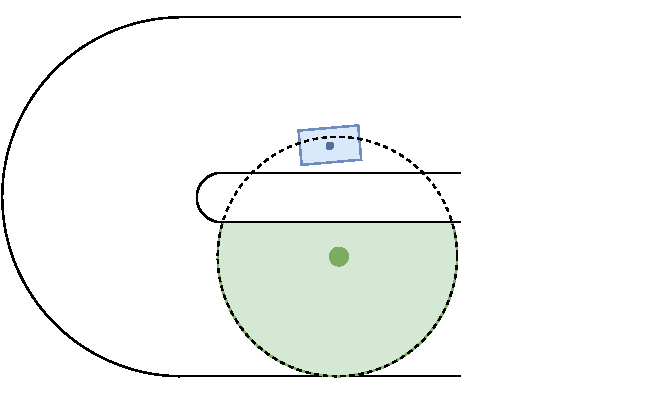
\includegraphics[width=\textwidth,trim=0 0 80 0, clip]{../img/waypoint_behind_wall}
	\caption{If the waypoint did not require direct visibility, the blue car would pass the waypoint whose radius is marked with the dashed line. The green area represents the actual waypoint area.}
	\label{fig:waypoints}
\end{figure}

To implement this goal condition, we must extend the state space $X$ with one extra discrete dimension. This dimension will denote how many waypoints the vehicle has passed since the initial state and we will define a function $\mu: X\rightarrow \mathbb{N}$ which returns this number. For the initial state $x_0$ the number of passed waypoints will always be 0. For a state $x\in X$ the value is defined based on the state from which it was reached $x'\in X$: 

\begin{equation*}
	\mu(x)=
	\begin{cases}
		\mu(x')+1 & x\in G_r(\vec{w_{\mu(x')+1}}) \\
		\mu(x') & otherwise.
	\end{cases}
\end{equation*}

The goal region $X_g$ will be a set of all states, which pass all $l$ waypoints:

\[
	X_g=\left\{x\in X \mid \mu(x)=l\right\}.
\]

\subsubsection{Problem Formulation}

In the previous sections, we described and defined the individual components of the trajectory planning problem. We can now formulate it formally:

\begin{defn}[Trajectory Planning Problem]

	A trajectory planning problem for a fast moving car is a tuple $\left(X, U_f, f_{\Delta t}, c, x_0, X_{\hat{w}}\right)$:

	\begin{itemize}
		\item A non-empty continuous set $X\subseteq\mathbb{R}^n$, which is the state space of the vehicle. Each state of the vehicle is represented by $n\in\mathbb{N}:n\geq4$ state variables and it contains the dimensions of the configuration of the vehicle in a two dimensional plane, a discrete dimension for the number of passed waypoints, and other state variables as defined by the vehicle model which is used.

		\item A non-empty finite set $U_f$ of actions, such that $\forall x\in X, \forall u\in U_f(x): c(f_{\Delta t}(x, u)) = F$, where $c$ is a collision detection function.

		\item A \textit{system simulator} $f_{\Delta t}:X\times U_f \rightarrow X$ for a fixed time period $\Delta t>0$.
		
		\item An initial state of the vehicle $x_0 \in X$.

		\item A goal region $X_g\subset X$ for some fixed sequence of waypoints \\ $\hat{w}=\langle w_0, w_1, w_2,\ldots, w_l \rangle, l>0$.
	\end{itemize}
\end{defn}

\subsubsection{Time-Optimal Feasible Solution}

The vehicle starts in an initial state $x_0$. It is controlled through an input sequence of actions applied over time at a constant rate, because we chose a fixed time interval $\Delta t>0$ between application of any two consequent actions. We can calculate the expected evolution of the state of the vehicle by integrating the velocity from a state transition function. If we take snapshots of the state every $\Delta t$ interval, we will get a sequence of states which we call a state trajectory:

\begin{defn}[Feasible State Trajectory]
	We say that a sequence of states $\hat{x_k}=\langle x_0,x_1,x_2,…,x_k \rangle ,x_i\in X$ is a feasible state trajectory starting in the state $x_0$ when for a fixed time interval $\Delta t>0$:
	\[
	\forall i \in \left\{ 0,\ldots,k-1\right\} \exists u\in U_f(x_i): x_{i+1}=f_{\Delta t} (x_i,u).
	\]
\end{defn}

We say that the state trajectory is feasible to emphasize the fact that it is collision-free. Remember that for each state $x$ we do not allow any actions which would lead to a crash to be in $U_f(x)$.

This sequence contains all the information we need to reconstruct the full continuous trajectory by finding the corresponding sequence of actions. In practice, this is not very important to us though. As we mentioned earlier, we do not expect the robot to be able to follow any plan perfectly, so we cannot execute the actions one by one. It is important for us to know in which the state the robot should at any given moment. The solution to our problem is therefore not a sequence of actions, but a state trajectory:

\begin{defn}[Feasible Solution]
	For an instance of a trajectory planning problem for a fast moving car $\left(X, U_f, f_{\Delta t}, c, x_0, g_{\hat{w}}\right)$, a feasible state trajectory $\hat{x_k}=\langle x_0, x_1, \ldots, x_k \rangle$ is a time-optimal feasible solution of the problem if:
	\begin{itemize}
		\item the final state is in the goal region: $x_k \in X_g$,
		\item and for every other feasible state trajectory $\hat{y_l}$, which ends in the goal region, it takes longer or the same time to reach the goal (i.e. $l \geq k$).
	\end{itemize}
\end{defn}

\paragraph{State Trajectory Sub-sampling}

The choice of the sampling time interval $\Delta t$ greatly impacts the performance of finding solutions to the planning problem. If the optimal time to reach the goal is $t$ seconds, then a state trajectory for a sampling interval $\Delta t_1$ will have more elements than a state trajectory with a sampling rate of $\Delta t_2 > \Delta t_1$. The planning algorithm would therefore have to make more decisions for $\Delta t_1$ and it would take longer to find a solution. On the other hand, a longer sampling interval could find invalid trajectories, because due to a long distance between two poses of the vehicle, the vehicle could ``jump through walls'' as the collision detection algorithm, which tests only the samples from the state trajectory, would give false positives.

Instead, we can uniformly subdivide the time interval of length $\Delta t$ into $n\in\mathbb{N}$ smaller intervals of $\Delta t/n$ and apply the state transition function $n$ times for every action in the sequence. This technique will give us better estimate of the motion of the vehicle and reduce the inaccuracy of numerical integration but at the same time it will not increase the computational complexity of the planning algorithm because we do not increase the number of explored sequences of actions. A good pair of $\Delta t$ and $n$ has to be found experimentally to provide good precision while keeping good performance of the algorithm on real hardware.

\section{Trajectory Planning Algorithms}
\label{sec:trajectory_planning_algorithms}

With a complete formulation of the trajectory planning problem for a fast moving car, we can design a planning algorithm which will find a time-optimal feasible solution trajectory starting at any given initial state and which will pass any sequence of waypoints it is given. Our planning algorithm must respect the differential constraints of our vehicle represented by the state transition function and avoid collisions with any obstacles by utilizing the collision detection function.

In this chapter we will introduce several well-known sampling-based algorithms and their variants which we considered for solving our trajectory planning problem. We will describe the main ideas behind these algorithms and discuss if and how they could be used in our specific use case.

\subsection{Rapidly-Exploring Random Trees (RRT)}

The \gls{RRT} is a simple randomized algorithm designed by Steven M. LaValle with differential constraints of mobile robots in mind \cite{RRT}. The core idea of this algorithm is to build a tree structure rooted in the initial state $x_0$ with branches representing state trajectories by randomly sampling the state space and using the system simulator function to find feasible trajectories in the state space.

The tree is grown iteratively by randomly sampling a state $x_{rand}\in X$ using some sampling scheme and choosing an action $u$ from $U_f$ which will steer the robot to a new state $x_{new}$ towards $x_{rand}$ without colliding with an obstacle from an existing tree node $x_{near}$ which is the closest to $x_rand$ according to some metric $\rho$ on $X$. The new node is added as a vertex to the tree and it is connected via an edge to its parent node $x_{near}$. This process is repeated until a state trajectory which ends in the goal region is found or until a fixed number of iterations is exceeded, in which case the search ends with a failure. The pseudocode of RRT is included in Algorithm~\ref{alg:rrt}.

\begin{algorithm}
	\SetAlgoLined
	\DontPrintSemicolon
	
	\SetKwFunction{AddVertex}{AddVertex}
	\SetKwFunction{AddEdge}{AddEdge}
	\SetKwFunction{TrajectoryFromBranch}{TrajectoryFromBranch}
	\SetKwFunction{SelectRandomSample}{SelectRandomSample}	
	\SetKwFunction{FindNearestNode}{FindNearestNode}
	
	\KwIn{Trajectory planning problem $(X, U_f, c, f_{\Delta t}, x_0, X_g)$, a metric on the state space $\rho$}
	\KwOut{State trajectory or $null$}
	\Parameter{Maximum number of iterations $K\in\mathbb{N}$}
	
	$T\gets \left(\left\{x_0\right\}, \emptyset\right)$\;
	
	\For{$k=1\ldots K$}{
		$x_{rand}\gets$ \SelectRandomSample{$X$}\;
		$x_{near}\gets$ \FindNearestNode{$T$, $x_{rand}$, $\rho$}\;
		$u_{best}\gets\argmin_{u\in U_f(x_{near})} \rho(x_{rand}, f_{\Delta t}(x_{near}, u))$\;
		$x_{new}\gets f_{\Delta t}(x_{near}, u_{best})$\;
		\AddVertex{$T$, $x_{new}$}\;
		\AddEdge{$T$, $\left(x_{near}, x_{new}\right)$}\;
		\If{$x_{new}\in X_g$}{
			\KwRet{\TrajectoryFromBranch{$T$, $x_{new}$}}\;
		}
	}
	
	\KwRet{null}\;
	
	\caption{The RRT algorithm.}
	\label{alg:rrt}
\end{algorithm}

\subsubsection{Algorithm Analysis}

\paragraph{Nearest Neighbor Search}

The algorithm performs a search for the closest state to the sampled state among the nodes in the tree according to the metric $\rho$ in every iteration of the algorithm and this search can have considerable impact on the performance of the algorithm.

A naïve solution would be to go over all tree nodes and find a node with minimum distance to the sampled state, but this approach would have linear time complexity with respect to the number of nodes of the tree. A better solution is to use a space partitioning data structure which is designed for nearest neighbor search. A good choice is a balanced $k$-d tree \cite{kd-tree}, where $k$ is the dimension of the partitioned space, in our case the dimension of $X$.

\paragraph{Time Complexity}

The algorithm will run for at most $K$ iterations. During every iteration, a random state will be sampled, nearest node will be found, an action will be selected, and the new state will be inserted into the already explored states tree structure.

We can assume that selecting a random sample of the state space does not depend on the already explored parts of the state space and that this operation time complexity is constant.

The complexity of finding the nearest neighbor and inserting a new node into a $k$-d tree with a fixed number of dimensions is logarithmic with respect to the number of nodes in the tree on average, in our case this means $O(\log K)$.

Finding an action which contributes to the largest progress towards the goal will be implemented by evaluating all the $m=|U_f|$ options and measuring the distance between the resulting state and the target state. The time complexity of this operation is $O(m)$.

Checking if a state is a goal state is a constant operation because we only have to check if $\mu{x_{new}}$ equals to the number of waypoints.

The time complexity of a single iteration of the algorithm is $O(\log K + m)$ and so the total time complexity of the algorithm is $O\left(K(\log K+m)\right)$.

\paragraph{Memory Complexity}

In order to capture the state of the algorithm, we need to keep the tree of all already explored states. As we discussed earlier, we use a $k$-d tree because of its nearest neighbor search queries. The memory complexity is linear with the number of nodes stored in the tree. In each iteration of the algorithm we add at most one new node to the tree which will lead to a tree with at most $K$ nodes. The memory complexity of the whole algorithm is therefore $O(K)$.

\paragraph{Completeness}

All nodes added to the tree are added as leaves and an edge between two nodes in the tree always corresponds to application of some action $u\in U_f$. None of the nodes added to the tree corresponds of a state which would collide with an obstacle.

All branches of the tree $T$ correspond to some feasible trajectory in the state space. The algorithm will stop as soon as the tree contains a branch which corresponds to a feasible solution trajectory or if the number of iterations exceeds the limit $K$.

\gls*{RRT} is proven to be probabilistically complete for $K$ approaching infinity \cite{RRT_star}. This means that if we sample the state space long enough and make our tree denser and denser, we are guaranteed to eventually find some solution. Because we chose the discrete-time model, we would have to also make the time discretization finer after each failure to achieve completeness.

\paragraph{Optimality}

The main difference between our modified algorithm and the original algorithm proposed by Steven LaValle is the early termination of the algorithm when the first solution is found \cite{RRT}. We do not try to find a better solution and we do not grow our tree in a way which would guarantee that the first solution we find will be an optimal solution.

\gls*{RRT} does not have any mechanism for finding optimal trajectories. On contrary, it is proven that the paths found by \gls*{RRT} are optimal with the probability of 0 \cite{RRT_star}.

There are modifications to the \gls*{RRT} algorithm which utilize the randomized sampling approach and probabilistic completeness of the algorithm, but which are optimal. One of these algorithms is called \gls{RRT*}. Unfortunately, this algorithm is not easily usable for us, because it is not designed for problems with differential constraints. The algorithm uses a ``rewiring'' procedure to optimize the tree edges after a new node is added. This procedure needs to be able to connect two states $x_1, x_2\in X$ with an action trajectory. This would be near impossible in the discrete-time model we chose and even with variable time, this operation would be very expensive and impractical.

\subsubsection{Sampling Schema}

The sampling schema is the most important part of the algorithm when it comes to the rate of convergence to a solution. The sampling function can also have an impact on the completeness of the algorithm.

\paragraph{Uniform sampling} is the simplest form of random node selection. The value for each dimension of the state vector is selected uniformly from the set of valid values.

\paragraph{Goal biasing} is a technique where we choose a state representing the final configuration with probability $p$ and we uniformly sample the space otherwise. This method can be generalized for several goals which can then be useful to bias the exploration of the state space in the direction of several waypoints. The goal of this method is to drive the search towards the goal faster, but at the same time keep the probabilistic completeness of the algorithm, as uniform sampling can help avoid getting stuck in dead ends.

\paragraph{Path biasing} is an extension of the goal biasing sampling scheme. We first find a reference path using a relaxed variant of the problem (e.g., a grid search algorithm without considering the differential constraints) and choosing the points along the path as intermediate goals for the grown tree. This variant of the algorithm is referred to as \textit{RRT-Path} \cite{RRT_guiding_path}.

\subsubsection{Conclusion}

The \gls*{RRT} is a very interesting algorithm. One of its biggest advantages is its simplicity. The algorithm is easy to understand and easy to implement. There are many extensions of the original idea which improve the rate of conversion to the goal. The algorithm is complete, if we allow it to search for a solution long enough. On the other hand, the algorithm finds a trajectory without any guarantee of optimality. The optimal extension of the algorithm \gls{RRT*} is hard to adapt to our use case, when we must consider the differential constraints of the vehicle.

\subsection{Hybrid A*}

Due to the infinite number of states reachable from an initial state $x_0\in X$ through actions from the infinite set of actions $U$ and the transition function $f_{\Delta t}$, it is impossible to exhaustively search for an optimal trajectory in the configuration space. Even if we limit the number of actions to a finite set of motion primitives $U_f$ and limit the maximum length of a trajectory, uninformed search for a trajectory will be impractically slow. In order to converge to a goal faster, informed search algorithms estimate graph nodes based on knowledge of the nature of the searched space.

A* is a complete and optimal informed graph search algorithm \cite{Nilsson_astar}. It visits the most promising nodes of the graph first, but it will eventually visit all the reachable nodes, until it finds a path to a goal state, or until every node was visited. We will describe a modified version of the A* algorithm which reduces the searched state space even further by discretizing the original continuous state space into an $n$-dimensional grid while still producing feasible trajectories in the configuration space.

This modified algorithm is referred to as \textit{Hybrid-State A* Search}. It was successfully used for path planning by the Stanford Racing Team in their vehicle \textit{Junior} during the DARPA Urban Challenge in 2007 \cite{dolgov08gppSTAIR}. This algorithm was utilized for navigation in unstructured environments when it was not possible to follow road center line such as parking lots and for other complex maneuvers such as U-turns or overtaking of other vehicles. It has been explored and successfully used by several other researchers since then \cite{Hybrid_astar}.

\subsubsection{State Space Discretization}

The advantage of A* is that it visits every state at most once and whenever we reach a graph node is visited, we have an assurance that the path through which we came from the initial node is the best possible one and we can ignore this node in the future if we find a different route to it. This works well for discrete search spaces where it is easy to compare two nodes between themselves and determine whether it was already visited or not. In a continuous state space, this can be problematic. Even though we come very close to an already visited node, it does not have to be equal to the node. Let us consider the following example.

\begin{example}
	Imagine we have a robot which moves in a two-dimensional plane and it is subject to differential constraints. The state space will be the configuration space $X=C$. We will focus on one action $u$ which moves the robot forward and steers to the left. In a fixed time of $\Delta t=1$ second the robot should travel around a quarter of a circle and turns by ninety degrees ($\dfrac{\pi}{2}$ radians). If we start from an initial state $x_0=\left(0,0,0\right)$ then after applying $u$ four times in a row, we would expect to go through states $x_1=\left(1,1,\dfrac{\pi}{2}\right),x_2=\left(0,2,\pi\right),x_3=\left(-1,1,\dfrac{3\pi}{2}\right)$, and arrive to a final state $x_4=\left(0,0,0\right)=x_0$ after 4 seconds. If we try to implement and run this example in a simulation, we might get a slightly different result caused by accumulated rounding errors and other numerical approximations. For example, we might use only a finite number of the decimals of the number $\pi$ and arrive to a heading angle of $\theta<2\pi$. The A* algorithm will consider $x_0$ and $x_4$ as different nodes of the graph and it will continue with the expansion of $x_4$. This example is visualized in Figure~\ref{fig:no_discretization_example}.
\end{example}

\begin{figure}
	\centering
	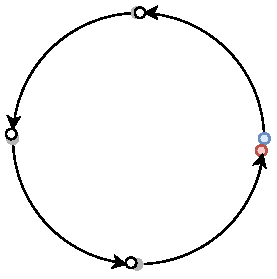
\includegraphics[width=0.5\textwidth]{../img/non_discretized_astar_state_duplication}
	\caption{We would expect the car to return to its initial position after the action $u$ was applied 4 times. Due to rounding errors and errors of numerical integration, we might reach a different state close to the initial state. The figure shows how the initial state, represented by the blue circle, gradually drifts from the expected position until it reaches the fourth state, represented by the red circle, which is different from the initial state.}
	\label{fig:no_discretization_example}
\end{figure}

\textit{Hybrid A*} divides the state space into a grid of similar states to avoid this problem. Before we expand a state from the configuration space, we will check if the grid cell it falls into is already closed or not. If the cell is closed, we will consider the state to be closed as well and we will not expand it again.

We can select an appropriate resolution for every dimension of the space base on the semantics of each dimension. If we wanted to ignore some dimension of the state space for searching, we can set the resolution for the dimension to $\infty$. We can convert the continuous dimensions of a state vector $x$ into a discrete grid coordinate with cell sizes vector $\vec{\sigma}$ with a state space discretization function $d: X\rightarrow X$:

\[
d(x) = \left\lfloor \dfrac{x}{\vec{\sigma}} \right\rfloor.
\]

The \textit{hybrid A*} algorithm stores the exact state through which we entered every visited discrete grid cell. The motion is continued by applying the action from the original continuous state, not the discretized one.

There is one problem with the discretization which is worth solving. Depending on the resolution of the grid, the next state obtained by the state transition function might fall into the same cell as the source state. This could be a significant problem especially at low speeds, for example when the vehicle is accelerating from a standstill. To solve this problem, we will repeat the same action $k$ times, until the resulting state falls into a different cell. We will then store the resulting state for future expansion with an appropriate cost.

\subsubsection{Heuristic Function}

The A* algorithm is driven towards the goal by a heuristic function. Designing a good heuristic function can help us converge towards the goal faster by expanding the most promising nodes first. The heuristic function estimates the remaining cost to go from any state to the goal. Our cost function represents time it takes to drive from one state to another. Our heuristic function therefore must estimate the remaining time it will take to reach the goal from a given state.

To guarantee optimality of A* for graph searching, we require the heuristic to be admissible and monotonous. This means that along any direct path from the initial node and a goal node the value of the heuristic must not increase and therefore maintain a form of triangle inequality.

The inspiration for our heuristic functions were taken from the Stanford Racing Team entry in the DARPA Urban Challenge \cite{dolgov08gppSTAIR}.

\paragraph{Euclidean Distance}
One of the simplest heuristics is calculating the distance between the position of the vehicle and the position of the goal. Our vehicle must drive past several waypoints. We must calculate the distance from the current position of the vehicle to the next waypoint and then add the distances between the remaining waypoints to obtain the minimum remaining distance $d$.

To calculate the time to reach the last waypoint, we must factor in the velocity of the vehicle. To maintain admissibility of the heuristic, we must assume that the vehicle will travel at maximum velocity. We will calculate the minimum time necessary by dividing the distance $d$ by the maximum possible velocity of the vehicle $v_{max}$.

This heuristic is admissible and monotonous, because as we move closer to the goal along any path, the Euclidean distance decreases and our estimate is always lower or equal to the real capabilities of our vehicle.

We ignore the driving characteristics of our vehicle and we also do not account for collisions with any of the obstacles or the boundary of the racing track. On the other hand, the value of the heuristic is easy to calculate, and it does not need any additional memory.

\paragraph{Shortest Path Through Waypoints}
We discretize the two-dimensional plane into a grid with the same resolution as we do for the position dimensions of the state space. We will then compute the distance to the goal in an eight-connected grid using dynamic programming. We ignore grid cells which are outside of the racing track or the ones which overlap with some obstacle. Given a distance, we can calculate the minimum time to reach the goal in the same way as in the case of Euclidean distance heuristic.

This heuristic ignores the capabilities of the vehicle and the constraints on steering. Nevertheless, it will guide the search along the course of the racing track, and it will help us avoid dead ends.

\paragraph{Combination of Heuristic Functions}
To take advantage of several different heuristics $h_1,h_2,\ldots ,h_n$, we can create a new heuristic, which takes the maximum estimated cost-to-go:
\[
h(x)=\max_{i \in {1, 2, \ldots, n}}h_i(x).
\]

This heuristic will dominate all the original heuristics and it will give us better estimates of the remaining cost. We will the combination of both the euclidean distance and shortest path heuristics as our final heuristic for the A* algorithm.

\subsubsection{Search Records}

We will conduct search over the state space of our vehicle. Besides the state vector, we need to remember additional information: the cost-to-come from the initial state to the current state and a pointer to the state from which we came to the current state. We will keep this information in records $\left(x, g, v_p\right)$, where $x\in X$ is the state, $g\in \mathbb{R}$ is the cost-to-come, and $v_p$ is the parent search record. The initial state does not have any parent search record. By traversing the search records, we can track back the states to the initial state and reconstruct the state trajectory which ends in any search record.

\paragraph{Cost-to-come} The cost of a trajectory accumulates over time and it is non-negative. The cost-to-come for the initial state is $0$. We fixed the time of execution of each action to $\Delta t$ seconds. If we start in a state with cost-to-come $g$ after applying an action $k\in \mathbb{N}$ times, the cost-to-come of the new state will be $g+k\Delta t$.

\subsubsection{Total Cost Estimate} The sum of the cost-to-come and the estimate of the cost-to-go from the heuristic function gives us an estimate of a total cost from the initial state to a goal state. The states with a lower total cost estimate are considered \textit{more promising} and we will explore these states first in order to speed up conversion to the goal region.

\subsubsection{Algorithm Analysis}

\begin{algorithm}[]
	\caption{The Hybrid A* algorithm.}
	\label{alg:hybrid_astar}
	
	\SetAlgoLined
	\DontPrintSemicolon
	
	\SetKwFunction{HybridAStar}{HybridAStar}
	\SetKwFunction{ReconstructTrajectory}{ReconstructTrajectory}
	\SetKwFunction{Expand}{Expand}
	\SetKwFunction{Open}{Open}	
	\SetKwFunction{Unfold}{Unfold}	
	
	\KwIn{Trajectory planning problem $(X, U_f, c, f_{\Delta t}, x_0, X_g)$, maximum trajectory cost limit $g_{max}$}
	\KwOut{State trajectory or $null$}
	\Parameter{State space discretization function $d: X\rightarrow X$, heuristic function $h$}
	
	\SetKwProg{algorithm}{Algorithm}{:}{}
	\SetKwProg{procedure}{Procedure}{:}{}
	
	\BlankLine
	
	\algorithm{\HybridAStar{$d$, $h$}}{
		$O\gets\left\{\left(x_0, 0, null\right)\right\}$\;
		$C\gets\emptyset$\;	
		\While{$O\neq\emptyset$}{
			$v\gets\argmin_{\left(x', g', v_p\right)\in O} g'+h(x')$\;
			$O\gets O\setminus\left\{v\right\}$\;
			\If{$x\in X_g$}{ \KwRet{\ReconstructTrajectory{$v$}}\; }
			$\left(x, g, v_p\right)\gets v$\;
			\If{$d(x) \notin C \land g < g_{max}$}{
				$C\gets C\cup\left\{d(x)\right\}$\;
				\Expand{$v$, $O$, $C$, $d$}\;
			}
		}	
		\KwRet{null}\;
	}
	
	\BlankLine
	
	\procedure{\Expand{$v$, $O$, $C$, $d$}}{
		\ForEach{$u\in U_f(x)$}{
			$\left(x, g, v_p\right)\gets v$\;
			$\left(x', k\right)\gets$ \Unfold{$x$, $u$, $d$}\;
			\If{$x' \neq \text{null} \land d(x')\notin C$}{
				$g'\gets g+k\Delta t$\;
				$O\gets O\cup\left\{\left(x', g', v\right)\right\}$\;
			}
		}
	}
	
	\BlankLine
	
	\procedure{\Unfold{$x_{start}$, $u$, $d$}}{		
		$\left(x_{last}, k\right)\gets \left(x_{start}, 0\right)$\;
		\Repeat{$x_{last}=x_{prev}\lor d(x_{start})\neq d(x_{last})$}{
			$x_{prev}\gets x_{last}$\;
			$x_{last}\gets f_{\Delta t}(x_{last}, u)$\;
			\lIf{$c(x_{last})=T$}{\KwRet{$\left(null, -1\right)$}}
			$k\gets k+1$\;
		}
		\KwRet{$\left(x_{last}, k\right)$}\;
	}
	
\end{algorithm}

In this section we will analyze the pseudo-code shown in Algorithm~\ref{alg:hybrid_astar}. We will explain how it differs from the original version of the A* algorithm \cite{Nilsson_astar} and we will then also analyze the time and memory complexity of the algorithm based on our choice of data structures.

The main procedure of the algorithm \texttt{HybridAStar} is very similar to what one could expect from the A* algorithm. We initialize an \textit{open set} $O$ with the initial state search record and also an empty \textit{closed set} $C$. We will say that a state is \textit{opened} if it has a record in $O$ and that it is \textit{closed} when the cell which it falls into is in $C$.

In the main loop, we obtain the most promising state $x\in O$ by comparing the total cost estimate of the open states. If $x$ reaches the goal region, we reconstruct the state trajectory by traversing the parent search records using a helper function \texttt{ReconstructTrajectory}. We test if the cell in which the state belongs has not been closed yet and only if it has not and the cost-to-come does not exceed the limit do we continue to expansion of the state. We close the cell into which the state $x$ belongs so that we will not expand any further states from this cell.

The expansion of a state is implemented in the procedure \texttt{Expand}. We try to explore the outcome of every possible action in $x$. We simulate the application of each action using the function \texttt{Unfold}. If the application of the action did not result in a collision, we will add the the final state $x'$ to $O$ if the cell $d(x')$, which was reached, has not been closed yet. In other versions of A*, it is common to check if the new state is currently in $O$. If $x'$ already is in $O$, in case when $x'$ was reached with a lower cost-to-come, the old $g$-value and the ancestor $p(x')$ would be replaced with the new values. We decided not to do this and instead keep both records in $O$. If any of these records for the same state are expanded before the algorithm finds a solution, its cell will be closed and so the consequent records of this state (with a higher cost-to-come), will be skipped when they are removed from the open set.

The simulation of the movement of the vehicle happens in the \texttt{Unfold} procedure. This function uses the system simulator function $f_{\Delta t}$ repeatedly until the vehicle stops (none of the properties of the vehicle state does not change after an action is applied), or until the vehicle leaves the cell of the parent state in the discretized state space.

\subsubsection{Time Complexity}

The time complexity of the A* algorithm depends mainly on the number of nodes which are expanded. We must also consider the complexity operations we perform whenever we expand a node. This involves an analysis of the way we implement the data structures for the open and closed nodes, which we vaguely expressed as set operations in the Algorithm~\ref{alg:hybrid_astar}.

\paragraph{The number of expanded states} The maximum length of a path in the search space we will explore is limited by the cost limit $g_{max}\in \mathbb{R}$. This limit alone defines a continuous bounded region of states which are reachable from the initial state. There are two factors, which affect the number of nodes that can be expanded: the discretization of time into $\Delta t$ second intervals and the discretization of the state space into a grid via the discretization resolution vector $\vec{\sigma}$. Both of these discretizations limit the number of states which are reachable. The total number of reachable states is then the minimum of these two limits.

Since our cost function is constant for all actions, we will only expand nodes at the ends of action sequences of at most $g_{max}/\Delta t$ steps. Due to the implementation of the \texttt{Unfold} procedure which might apply a single action multiple times in a row, the length of the sequence and therefore the number of expanded nodes can be even smaller. The expanded nodes form a tree with at most $l=\left\lceil g_{max}/\Delta t\right\rceil$ levels with a branching factor of $b=|U_f|$. Each of the states $x$ will be expanded at most once, because if it were to be expanded the second time, its cell would already be closed ($d(x)\in C$). This means that in the worst case when there are no obstacles and each state would be in a different cell, the number of expanded nodes would be $O(b^l)$.

The number of reachable states in the discretized state space also limits the number of expanded states, as at most one state will be expanded per each discrete cell. If the state space has $d$ dimensions and the maximum number of discrete cells in the individual dimensions is $\vec{n}=\left(n_1, n_2, \ldots, n_d\right)\in \mathbb{N}^d$, the upper limit for the number of cells is $\max(\vec{n})^d$.

\paragraph{Open set operations} In order to keep track of which element should be expanded next, we need to keep the data in the open set arranged in a priority queue by their total cost estimate $g+h(x)$. We use three operations of the priority queue: adding an element, and getting and removing an element with the minimum key. When implemented as a binary heap, all of these operations will have time complexity of $O(\log n)$, where $n$ is the number of nodes in the queue\footnote{The complexity of insertion can be reduced to constant time with an advanced heap, such as a binomial or Fibonacci heap. The choice of the binary heap is motivated by the priority queue in the C++ STL, which implements a binary heap.}. This can be at most $b^l$ and so the time complexity would be $O(\log b^l)=O(l \log b)$.

\paragraph{Closed set operations} In order to keep track of all the cells which have been closed, we need a data structure with an efficient insertion and element retrieval operation. This can be achieved with a hash table with an amortized time complexity of $O(1)$.

\paragraph{Heuristic function} Our heuristic function is implemented as a maximum of several heuristics, which can all be implemented as lookup tables and so the time complexity will be $O(1)$.

\paragraph{The \texttt{Unfold} procedure}
The time complexity of ``unfolding`` depends on the number of repetitions of the action, before the state leaves the original cell. Each evaluation of the system simulator function $f_{\Delta t}$ is a non-trivial operation, which includes numerical integration, but asymptotically this operation is still $O(1)$. The collision detection function performs a single query into the occupancy grid with inflated obstacles. This is a simple operation with the complexity of $O(1)$. We will assume that in most cases, the number of repetitions is low and it is bound by some small constant. We will assume that the \texttt{Unfold} procedure as a whole is constant.

\paragraph{The \texttt{Expand} procedure}
The expansion tries to apply all of the available actions and adds all collision-free extensions of the previous state to the open set, unless the cell is already closed. For each action, we call the \texttt{Unfold} procedure, check if an element is already in the closed set, and we may insert an element into the open set. This gives us a total time complexity of $O(bl \log(b))$.

\paragraph{Total time complexity} For we get each expanded state from the heap and run the \texttt{Expand} procedure. The total time complexity is therefore $O(b^l \cdot l\log b \cdot bl \log b)=O(l^{2}b^{l+1}\log^2 b)$. The dominating factor is the exponential $b^{l+1}$. This is expected, because motion planning was shown to be PSPACE-hard \cite[Chapter~6.5.1]{lavalle_2006}.

\subsubsection{Memory Complexity}

Each of the states requires only a constant amount of memory. The only additional information stored in memory are the lookup tables of the heuristic functions which require at most linear space in the size of the discretized search space, which is at most $O(b^l)$. The graph itself does not have to be explicitly held in memory as we traverse it through calling the system simulator. The memory complexity of the open set $O$ (implemented as a priority queue) and the closed set $C$ (implemented as a hash table) is linear with the number of items stored in the data structure. The number of open or closed nodes can be at most the number of all expanded states. The memory complexity of the algorithm in the worst case is therefore $O(b^l)$.

\subsubsection{Conclusion}

The \textit{Hybrid A*} algorithm is a good option for trajectory planning. The size of the state space is enormous and the heuristic function helps us to focus on the most promising directions first and only explore the seemingly bad trajectories if we run to a dead end. The algorithm is systematic and if a solution exists, it will eventually find it. The order in which the algorithm explores the state space gives us a guarantee that the first solution it will find will be the optimal solution. The selected discretization of time $\Delta t$ and of the size of the cells of the state space $\vec{\sigma}$ can have an impact on the existence of a solution. In theory, by making the discretization finer, we are guaranteed to find a solution. In practice, we could fine-tune the size of the cells $\vec{\sigma}$, to balance the performance and the ability to find solutions during the first search in most cases.

\subsection{Space Exploration Guided Heuristic Search (SEHS)}

Chao Chen presents a different approach to the discretization of the state space. In his dissertation, he presents a novel \gls{SEHS} algorithm and several extensions of this algorithm \cite{SEHS}. The author points out that for systems subject to nonholonomic constraints, uniform discretization is suboptimal. Instead, a guidance path consisting of overlapping circles with their centers on the circumferences of each other and with their radii based on the distance to the nearest obstacle from the start position to goal region is found. The path is then used as a heuristic to guide the search and the circles are used to discretize the position dimensions of the state space as a Voronoi diagram around the centers of these circles. This algorithm reduces the number of expanded nodes when compared to both \gls*{RRT} or \textit{Hybrid A*}, which is demonstrated by the author on a series of experiments. In this section, we will describe this search method more in depth.

\subsubsection{Space Exploration (SE)}
\label{sec:space_exploration}

Space exploration is a pre-processing step of the planning algorithm. We are looking for the shortest path of overlapping circles in $\mathbb{R}^2$ form the initial state position to the goal location. The centers of each circle lies on the circumference the previous circle along the path. The radii of the circles are in some closed interval $\left[r_{min}, r_{max}\right]\subset \mathbb{R}_{>0}$ and each radius is chosen so that it is as large as possible, but none of the circles can overlap a cell with an obstacle in the occupancy grid map of the track. The path of circles does not give us only the shortest path from the initial state to a goal.

The exploration step can be implemented with a basic \textit{A*} search starting at the initial state location. During the expansion step of \textit{A*}, we will create a fixed number of new circles $n\in \mathbb{N}$ evenly spaced on the circumference of the expanded circle. The radius for each new circle will be calculated by measuring the distance to the closest obstacle and trimming this value to be within the interval of accepted radii. We will not open any circles with a smaller radius than $r_{min}$. The search will end once we expand a circle which includes some endpoint $\vec{x_{goal}}\in \mathbb{R}^2$. The cost function will be the length of the path measured by the distances between the centers of the circles, which is incidentally just the sum of the radii of the circles along the path. The heuristic function $h_{\vec{x_{goal}}}$ will be a simple euclidean distance between the center of a circle and the goal point $\vec{x_{goal}}$.

Our goal is defined by a sequence of waypoints. We will start from the position of the initial state and use the center of the first waypoint as a goal. From the final circle in this path, we will run the algorithm again with the center of the second waypoint as a goal. The result will be a path through all of the waypoints, which is exactly what we need.

\begin{algorithm}[]
	\caption{The Space Exploration algorithm.}
	\label{alg:space_exploration}
	
	\SetAlgoLined
	\DontPrintSemicolon
	
	
	\SetKwFunction{SpaceExploration}{SpaceExploration}
	\SetKwFunction{FindPathBetween}{FindPathBetween}
	\SetKwFunction{Expand}{Expand}
	\SetKwFunction{DistanceToClosestObstacle}{DistanceToClosestObstacle}
	\SetKwFunction{ReconstructTrajectory}{ReconstructTrajectory}
	\SetKwFunction{PointsOnCircumference}{PointsOnCircumference}
	
	\KwIn{Occupancy grid $O_r^{m\times n}$, initial position $\vec{x_0}\in\mathbb{R}^2$, list of waypoints $\hat{w}=\left\langle \vec{w_1}, \vec{w_2}, \ldots, \vec{w_l} \right\rangle\in\mathbb{R}^l$, range of valid radii $\left[r_{min}, r_{max}\right]\subset\mathbb{R}_{>0}$, number of child circles $n\in\mathbb{N}$.}
	\KwOut{Path of circles or $null$}
	
	\SetKwProg{algorithm}{Algorithm}{:}{}
	\SetKwProg{procedure}{Procedure}{:}{}
	
	\BlankLine
	
	\algorithm{\SpaceExploration{$O_r^{m\times n}$, $\vec{x_0}$, $\hat{w}$, $\left[r_{min}, r_{max}\right]\subset\mathbb{R}_{>0}$, $n\in\mathbb{N}$}}{
		$\vec{x_{start}}\gets \vec{x_0}$\;		
		\For{$i=1\ldots l$}{
			$c_i\gets $ \FindPathBetween{$\vec{x_{start}}$, $\vec{w_i}$}\;
			\lIf{$c_i=\text{null}$}{ \KwRet{null} }
			$\vec{x_{start}}\gets \text{center of last circle of } c_i$\; 
		}
		\KwRet{$c_1+c_2+\ldots +c_l$}\;
	}
	
	\BlankLine
	
	\procedure{\FindPathBetween{$\vec{x_{start}}$, $\vec{x_{goal}}$}}{
		$r_{start}\gets $ \DistanceToClosestObstacle{$O_r^{m\times n}$, $\vec{x_{start}}$, $r_{max}$}\;
		$O\gets\left\{\left(\vec{x_{start}}, r_{start}, 0, null\right)\right\}$\;
		$C\gets\emptyset$\;
		\While{$O\neq\emptyset$}{
			$v\gets\argmin_{\left(\vec{x'}, r', g', v_p\right)\in O} g'+h_{\vec{x_{goal}}}(\vec{x'})$\;
			$O\gets O\setminus\left\{v\right\}$\;
			$\left(\vec{x}, r, g, v_p\right)\gets v$\;
			\If{$\norm{\vec{x}-\vec{x_{goal}}}<r$}{ \KwRet{\ReconstructTrajectory{$v$}}\; }
			\If{$\forall \left(\vec{x'}, r'\right) \in C: \norm{\vec{x}-\vec{x'}}\geq r'$}{
				$C\gets C\cup\left\{\left(\vec{x}, r\right)\right\}$\;
				\Expand{$v$, $O$, $C$}\;
			}
		}	
		\KwRet{null}\;
	}
	
	\BlankLine
	
	\procedure{\Expand{$v$, $O$, $C$}}{		
		$\left(\vec{x}, r, g, v_p\right)\gets v$\;
		\ForEach{$\vec{x'}\in $ \PointsOnCircumference{$n$, $\vec{x}$, $r$}}{
			$r'\gets $ \DistanceToClosestObstacle{$O_r^{m\times n}$, $\vec{x'}$,  $r_{max}$}\;
			\If{$r' \geq r_{min} \land \forall \left(\vec{x''}, r''\right) \in C: \norm{\vec{x'}-\vec{x''}}\geq r''$}{
				$g'\gets g+r$\;
				$O\gets O\cup\left\{\left(\vec{x'}, r', g', v\right)\right\}$\;
			}
		}
	}
\end{algorithm}

The pseudo-code of space exploration is shown in Algorithm~\ref{alg:space_exploration}. The main method ``stitches'' together the path from paths between the individual waypoins, which are obtained using the \texttt{FindPathBetween} procedure. This procedure implements the space exploration algorithm itself. It is an implementation of the standard A* algorithm and it shares most of the logic with Algorithm~\ref{alg:hybrid_astar}. There are only a few aspects, which deserve additional commentary:

\begin{enumerate}
	\item A point is considered to be \textit{closed}, when it is an internal point of an already expanded circle. This is not a simple operation which could be implemented using a hash-table. We can assume that we would perform a check against every circle in $C$ and so the complexity would be linear with the size of $C$.
	
	\item The function \texttt{PointsOnCircumference} calculates $n$ polar coordinates $p_i=(2\pi i/n, r)$, where $r$ is the given radius, and converts them into Cartesian coordinates with respect to the given center of the circle.
	
	\item We implement the \texttt{DistanceToClosestObstacle} function by generating a fixed number of rays around the starting point and using a ray-marching algorithm to find the distance along the ray at which we enter a cell which is occupied by an obstacle. The number of rays must be high enough so that the risk of missing an obstacle between two rays within the radius $r_{max}$ is low. We assume that the obstacles marked in the map are fairly large and that their surfaces are smooth, without long spikes. This approach is inspired by the way a \gls{LIDAR} works.
\end{enumerate}

The path of circles can be further optimized to find a shorter path between the centers of the circles, while not reducing the clearance from obstacles. The space exploration algorithm might not find the shortest path, because it considers only a fixed number of directions when a circle is expanded. The author of the algorithm proposes a simple iterative algorithm which adjusts the center of each circle $(\vec{x_i}, r_i)$ to be on the line between $\vec{x_{i-1}}$ and $\vec{x_{i+1}}$ in the ratio of $r_{i-1}:r_{i+1}$, if the distance to the nearest obstacle from this point is greater or equal to $r_i$. This process is repeated until some of the circles can be adjusted. At the end of these adjustments, the centers of the circles might not be on the circumferences of other circles, but the circles will still be overlapping. The single optimization step is visualized in Figure~\ref{fig:sehs_space_exploration_optimization} and further details of this process are described in~\cite[Section 2.2.3]{SEHS}.

\begin{figure}
	\centering
	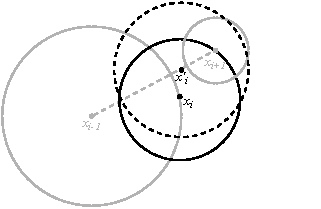
\includegraphics[width=0.5\textwidth]{../img/se_optimization_step}
	\caption{The optimization step of the path of circles moves the center of a circle only if the length of the path through the centers of the circles decreases and the radius of the circle can be increased or it stays the same. The center of the new circle might not be placed on a circumference of another circle.}
	\label{fig:sehs_space_exploration_optimization}
\end{figure}

\subsubsection{Heuristic Search (HS)}

The second phase of the \gls*{SEHS} algorithm is identical to \textit{Hybrid A*} as we defined it in Algorithm~\ref{alg:hybrid_astar}. We must only define a state space discretization function $d_{SEHS}: X\rightarrow X$ and a heuristic function $h_{SEHS}: X\rightarrow \mathbb{R}$. Both of these parameters will be derived from the path of circles obtained from the pre-processing phase.

\paragraph{State Space Discretization}
We will use the centers of the circles $X_c=\left\{\vec{c_1}, \vec{c_2}, \ldots, \vec{c_k} \right\}, \vec{c_i}\in\mathbb{R}^2$ obtained from the pre-processing to define the discretization of the $x$ and $y$ dimensions of the configuration space $C$. Any point $\vec{x}\in \mathbb{R}^2$ will be projected on the closest circle in $X_c$. The function $d_{x,y}:\mathbb{R}^2\times X_c$ effectively defines the Voronoi diagram:

\begin{equation*}
\begin{aligned}
i(\vec{x})&=\argmin_{j\in \left\{1, 2, \ldots, k\right\}} \norm{\vec{x}-\vec{c_j}} \\
d_{x,y}(\vec{x})&=c_{i(x)}.
\end{aligned}
\end{equation*}

Determining which center of a circle $\vec{c_i}$ is closest to a point $\vec{x}$ is an instance of a nearest-neighbor problem, which we already discussed when we described the RRT algorithm. It turned out that simple linear search is more efficient than a space-partitioning data structure when we ran the algorithm. This is most likely due to the fact that the number of circles $k$ was usually low and that the array of all waypoints can be loaded into the cache of a processor and it does not require any expensive branching operations, unlike a search in a tree.

The path of circles does not give us any information which could be used to discretize the heading angle of the vehicle $\theta$ or any other additional state variables. For these state variables, we have to use the same uniform cell discretization as in \textit{Hybrid A*}.

This space discretization has one big advantage over the uniform grid discretization. When the path goes through a long wide corridor, it will consist of a small number of circles with large radii. Going through this part of the track will not require too many control inputs. When the path goes through a narrow passage between obstacles or through a corner, the radii of the circles will be smaller and so the number of circles in this area will be larger. Going through this region will probably require finer control over the vehicle. We will be able to explore more different control input sequences through this area because the discretization will be denser here.

\paragraph{Heuristic}
The heuristic function estimates the remaining time which it could take to reach the goal. As in \textit{Hybrid A*}, we will estimate the remaining distance from the current state to the goal region and divide this distance by the maximum possible velocity of the vehicle $v_{max}$. For some point $\vec{x}\in \mathbb{R}^2$ we will find the circle closest to it and add the distance to the center of the next circle and the sum of the distances between the rest of the circles until the end region:

\begin{equation*}
\begin{aligned}
m(\vec{x})&=\norm{\vec{x}-\vec{c_{i(\vec{x})+1}}}+\sum_{j=i(\vec{x})+1}^{k-1} \norm{\vec{c_j}-\vec{c_{j+1}}} \\
h(\vec{x})&=\dfrac{m(\vec{x})}{v_{max}}.
\end{aligned}
\end{equation*}

\subsubsection{Conclusion}

The \gls*{SEHS} algorithm is a simple yet efficient way of searching a state space for a car-like vehicle. It promises significantly faster convergence towards a solution than \textit{Hybrid A*}, but the implementation itself is very similar. The main difference is in the discretization of the state space, which is much denser when the desired path is near obstacles and less dense when there are no obstacles around. We will implement both \textit{Hybrid A*} and \gls*{SEHS} and compare the results of these two algorithms.

\section{Track Segmentation}
\label{sec:track_segmentation}

A natural way of splitting the track into smaller segments is to find the corners of the track. We can then plan the trajectory for the very next turn in front of the vehicle and for one or two  consecutive ones, and imitate the behavior of a human racing driver, as we described it in Section~\ref{sec:racing_line}. To prevent long segments for long straight stretches, we can set a limit for the length of a segment and split long segments into multiple shorter ones.

Another benefit of splitting the track into smaller segments and planning the trajectory just for a fixed number of them is that the total length of the track does not affect the performance of the algorithm anymore. The length of the segments is limited and so the actual time it will take to calculate a trajectory for the next $n$ segments on real hardware should be similar for different parts of the track. We will have to test this hypothesis experimentally.

In this section we will describe an algorithm we chose to find points close to corners of a racing circuit. We will use this algorithm just once before a race starts.

The definition of a racing circuit as an occupancy grid $O_r^{m\times n}$, initial configuration of the vehicle $c_0\in C$, and a sequence of at least two checkpoints $\vec{p_i}\in\mathbb{R}^2$ which defines the direction in which the vehicle has to drive along the circuit and which parts of the grid it should go through in the case when there are multiple ways to reach a goal or of the track intersects itself at some point. The question is, how do we find a corner of a track in an occupancy grid? We can make a simple observation and derive an algorithm which will produce good approximate solutions.

Intuitively, a corner is point where the track bends and we are not able to keep driving in a straight line anymore. We can relax our problem for a moment and imagine, that robot has a differential drive. This allows it to move straight in the direction where it is heading, then stop, rotate around its vertical axis, and then start moving in the new direction. If we found a collision-free path for this robot in the occupancy grid through all the checkpoints of the track, the pivot points of the robot would be in the vicinity of the corners. It might be possible that it would require several turns within a short distance of each other to go around the corner, (e.g., a so-called ``hairpin'' corner as shown in the bottom left corner of Figure~\ref{fig:corner_detection_hairpin_corner}) and so not every change of direction could be simply interpreted as a corner and some of them should be merged.

We will implement an algorithm based on this thought experiment which will have three steps:
\begin{itemize}
	\item We will find the pivot points in a path for the differential drive robot through the occupancy grid which starts at the initial position of the vehicle and which goes through the checkpoints.
	\item We will eliminate pivot points, where the direction does not change significantly.
	\item We will find clusters of the remaining pivot points along the path and keep only one of them, this point will be one of the final waypoints.
\end{itemize}

\begin{figure}[]%
	\centering
	\begin{subfigure}[b]{0.49\textwidth}
		\centering
		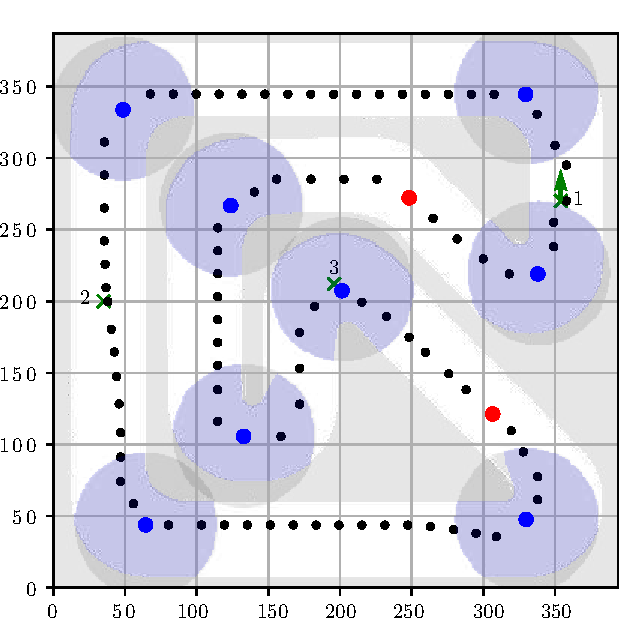
\includegraphics[width=\textwidth]{../img/track-analysis/race_track}
		\caption{Circuit ``U''}
	\end{subfigure}
	\hfill
	\begin{subfigure}[b]{0.49\textwidth}%
	\centering
	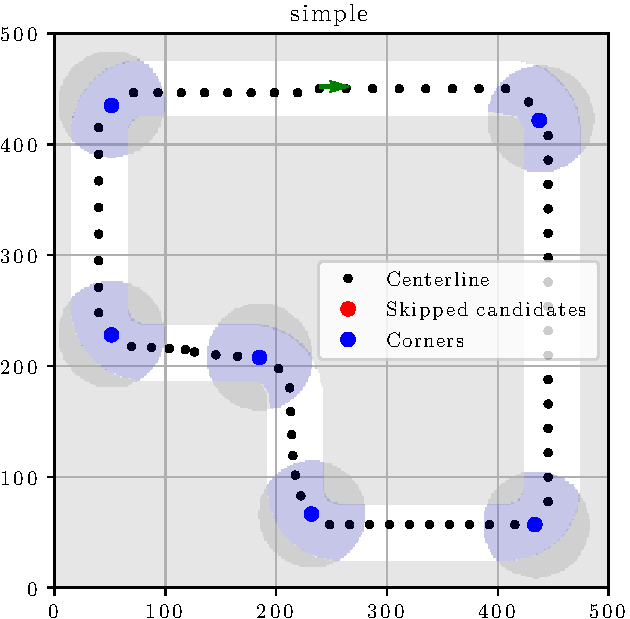
\includegraphics[width=\textwidth]{../img/track-analysis/simple}
	\caption{Circuit ``Simple''}
	\end{subfigure}
	\vskip\baselineskip
	\begin{subfigure}[b]{0.49\textwidth}
		\centering
		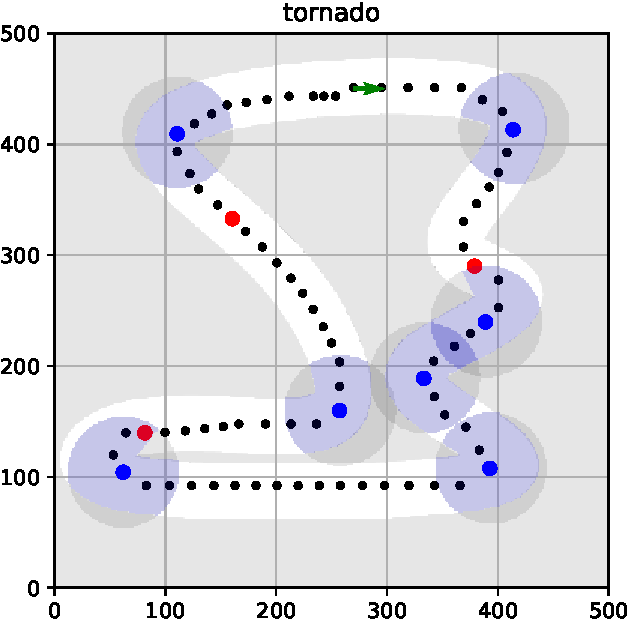
\includegraphics[width=\textwidth]{../img/track-analysis/tornado}
		\caption{Circuit ``Tornado''}
		\label{fig:corner_detection_hairpin_corner}
	\end{subfigure}	
	\hfill
	\begin{subfigure}[b]{0.49\textwidth}
		\centering
		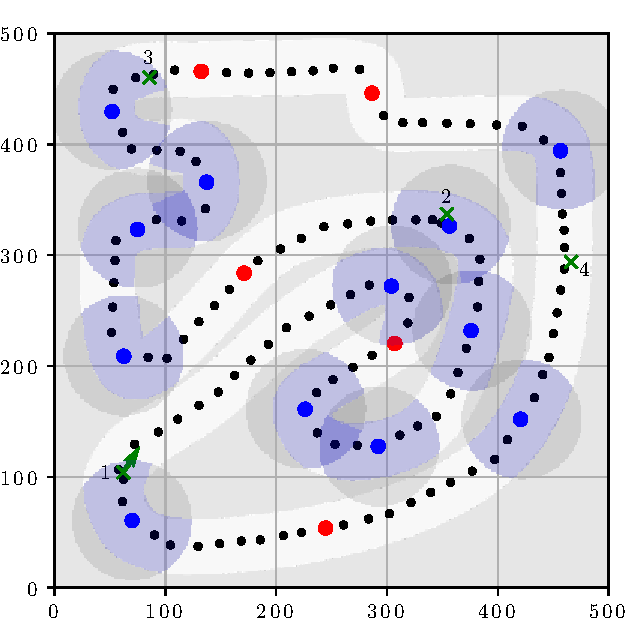
\includegraphics[width=\textwidth]{../img/track-analysis/zurich}
		\caption{Circuit ``Zurich''}
	\end{subfigure}
	
	\label{fig:corner_detection}
	\caption{This figure shows several different tracks on which we applied the track segmentation algorithm. The tracks have different layouts and feature different density and types of corners. The blue circles represent the detected corners.}
\end{figure}


\subsection{Finding Pivot Points}
The shortest path can be found in several different ways. We can reuse the \textit{Space Exploration} algorithm which was described in Section~\ref{sec:space_exploration}. The final path will consists of steps where the robot picks one of the fixed number of possible directions, and it will move forward in this direction, before it picks another direction. If we set the minimum radius of the circles to the half of the track width, then we will find a line resembling a center line of the track. Because the width of the track can vary along the circuit, we allow the radii of the circles to be between \SI{60}{\percent} and \SI{200}{\percent} of half of the width of the track at the starting position.

\begin{algorithm}[]
	\caption{Find Pivot Points}
	\label{alg:find_pivots}
	
	\SetAlgoLined
	\DontPrintSemicolon
	
	\SetKwFunction{FindPivotPoints}{FindPivotPoints}
	\SetKwFunction{SpaceExploration}{SpaceExploration}
	\SetKwFunction{ProcessNext}{ProcessNext}
	\SetKwFunction{CorrectTailToHeadConnection}{CorrectTailToHeadConnection}
	
	\KwIn{Occupancy grid $O_r^{m\times n}$, initial state $x_0$, directly visible points relation $O_r^{m\times n}$, sequence of checkpoints $\hat{p}_k=\left\langle \vec{p_1}, \vec{p_2}, \ldots, \vec{p_k} \right\rangle$}
	\KwOut{Sequence of pivot points}
		
	\SetKwProg{algorithm}{Algorithm}{:}{}
	\SetKwProg{procedure}{Procedure}{:}{}
		
	\BlankLine
	
	\algorithm{\FindPivotPoints{$O_r^{m\times n}$, $x_0$, $\hat{p}_k$, $r_{track}$}}{
		$\hat{q}_l\gets $ \SpaceExploration{$O_r^{m\times n}$, $\kappa_{x,y}(x_0)$, $\hat{p}_k$, $\left[0.6 r_{track}, 2 r_{track}\right]$}\;
		$W\gets \emptyset$\;
		$i_{last}\gets 1$\;
		\ForEach{$i\in \left\{2,3,\ldots,l\right\}$} {
			$(W, i_{last})\gets $ \ProcessNext{$W$, $i_{last}$, $i$}\;
		}
		\KwRet{subsequence $\hat{w}_m\subseteq\hat{q}_l: m=|W| \land \forall q_i\in \hat{w}_m: i\in W$}
	}

	\BlankLine

	\procedure{\ProcessNext{$W$, $i_{last}$, $i$}}{
		\If{$\left(\vec{q_{i_{last}}}, \vec{q_i}\right)\notin D(O_r^{m\times n})$}{
			$i_{last}\gets i-1$\;
			$W\gets W\cup\left\{ i_{last} \right\}$\;
		}
		\KwRet{$(W, i_{last})$}\;
	}
\end{algorithm}

The outcome of the \texttt{FindPivotPoints} algorithm, the pseudo-code of which is shown in Algorithm~\ref{alg:find_pivots}, is a sequence of pivot points such that two adjacent points in the sequence are \textit{directly visible} and the distances between these points are as long as possible. We use the \texttt{SpaceExploration} algorithm to find the ``center line'' $\hat{q}_l$ consisting of $l$ points. We then go around the track and we try to merge these steps into longer straight lines.

We start from the initial position and pretend that this is the last marked pivot point. We find the furthest point along $\hat{q}_l$, which is directly visible from the last waypoint, and mark it as an index of the next waypoint. We then repeat this process from next waypoint until we reach the end of the track.

\paragraph{No Obstacles Edge Case} In the case, when there are no obstacles in the occupancy grid, then all of the points will be visible from each other and the whole sequence would collapse into a single waypoint. We will ignore this edge case and assume that the racing circuit has a non-trivial layout.

\subsection{Estimating Positions of Corners}

Once we have a sequence of pivot points, we can estimate the positions of corners based on these pivot points. Whenever the track curves, we expect a pivot point in the vicinity.

At some pivot points, the direction of the robot changes only very little. This means, that the angle between the previous point, the current point, and the next point along the path, will be close to $\pi$. The first pass of our algorithm removes pivot points, at which the angle is above some angle threshold value $\alpha_{max}$. To calculate the angle between three consecutive points along the path $\vec{p_{i-1}}, \vec{p_i}, \vec{p_{i+1}}\in\mathbb{R}^2$, we use the law of cosines to calculate the angle between the vectors $\vec{x}=\vec{p_{i-1}}-\vec{p_i}$ and $\vec{y}=\vec{p_{i+1}}-\vec{p_i}$:

\[
	\alpha(\vec{x}, \vec{y})=\arccos \left(\dfrac{\vec{x}\cdot\vec{y}}{\norm{\vec{x}}\norm{\vec{y}}}\right),
\]

where $\cdot$ represents the scalar product between the two vectors.

It might be possible, that the \texttt{FindPivotPoints} algorithm returns a path, where there are several pivot points close to each other. We will try to merge these close pivot points into a single point, to reduce the number of very short segments. This complete algorithm is summarized as pseudocode in Algorithm~\ref{alg:find_corners}.

\begin{algorithm}[]
	\caption{Find Corners}
	
	\SetAlgoLined
	\DontPrintSemicolon
	
	\SetKwFunction{FindCorners}{FindCorners}
	\SetKwFunction{MergeClosePoints}{MergeClosePoints}
	\SetKwFunction{CloseNeighbors}{CloseNeighbors}
	\SetKwFunction{Walk}{Walk}
	\SetKwFunction{Next}{Next}
	\SetKwFunction{Prev}{Prev}
	\SetKwFunction{SelectSubsequenceBySkipping}{SelectSubsequenceBySkipping}
	
	\KwIn{Sequence of points $\hat{p}_k=\left\langle \vec{p_1}, \vec{p_2}, \ldots, \vec{p_k} \right\rangle$, minimum distance between corners $d_{min}\in\mathbb{R}_{>0}$}
	\KwOut{Sequence of locations of corners}
	\Comment{We will use the notation $\vec{p_{i-1}}$ and $\vec{p_{i+1}}$ to reference the previous and next point of the $i$-th point in the sequence. The sequence of points represents a loop. The previous point for $\vec{p_1}$ is the very last point $\vec{p_k}$ and the next point after $\vec{p_k}$ is $\vec{p_1}$. }
	
	\SetKwProg{algorithm}{Algorithm}{:}{}
	\SetKwProg{procedure}{Procedure}{:}{}
	
	\BlankLine
		
	\algorithm{\FindCorners{$\hat{p}$, $\alpha_{max}$, $d_{min}$}}{
		$R\gets \left\{i\in\left\{1,\ldots,|\hat{p}|\right\}\mid \alpha(\vec{p_{i-1}}-\vec{p_i},\vec{p_{i+1}}-\vec{p_i})>\alpha_{max}\right\}$\;
		$\hat{p}'\gets $ \SelectSubsequenceBySkipping{$\hat{p}$, $R$}\;
		\KwRet{\MergeClosePoints{$\hat{p}'$, $d_{min}$}}\;
	}
	
	\BlankLine
	
	\procedure{\MergeClosePoints{$\hat{p}$, $d_{min}$}}{
		$\hat{p}'\gets \hat{p}$\;
		\Repeat{$\hat{p}'\neq\hat{p}$}{
			$\hat{p}\gets\hat{p}', k\gets |\hat{p}|$\;
			$i_{max}\gets \argmax_{i\in \left\{1,\ldots,k\right\}} |$\CloseNeighbors{$i$, $\hat{p}$, $d_{min}$}$|$\;
			$N\gets $ \CloseNeighbors{$i_{max}$, $\hat{p}$, $d_{min}$}\;
			$i_{corner}\gets \argmin_{i\in N} \alpha(\vec{p_{i-1}}-\vec{p_i}, \vec{p_{i+1}}-\vec{p_i})$\;
			$\hat{p}'\gets $ \SelectSubsequenceBySkipping{$\hat{p}$, $N\cup\left\{i_{max}\right\}\setminus\left\{i_{corner}\right\}$}\;
		}
		\KwRet{$\hat{p}$}\;
	}

	\BlankLine

	\procedure{\CloseNeighbors{$i$, $\hat{p}$, $d_{min}$}}{
		$N_{ahead}\gets $ \Walk{$i$, $\hat{p}$, $d_{min}$, $i\mapsto i-1$}\;
		$N_{after}\gets $ \Walk{$i$, $\hat{p}$, $d_{min}$, $i\mapsto i+1$}\;
		\KwRet{$N_{ahead}\cup N_{after}$}\;
	}

	\BlankLine

	\procedure{\Walk{$i$, $\hat{p}$, $d_{min}$, $f_{step}$}}{
		$N\gets\emptyset$\;
		$j\gets f_{step}(i)$\;
		\While{$\norm{\vec{p_i}-\vec{p_j}}<d_{min}\land j\neq i$}{
			$N\gets N\cup\left\{j\right\}$\;
			$j\gets f_{step}(j)$\;
		}		
		\KwRet{$N$}\;
	}

	\label{alg:find_corners}
\end{algorithm}

\subsubsection{Algorithm Analysis}

The algorithm will always be complete and return a sequence of points such that for any of two consecutive points the distance between these points is at least $d_{min}$. 

If during an iteration in \texttt{MergeClosePoints} no two consecutive points which are closer than $d_{min}$ are found in $\hat{p}$, the algorithm stops. If at least one cluster of points is merged, then at least two points from the original sequence are removed and only one point is added. In every iteration the length of the sequence therefore decreases. After at most $k-1=|\hat{p}|-1$ iterations, the number of points in the sequence will drop to a single point, and the algorithm will stop.

In every iteration, we find the biggest cluster of points along the sequence and we find the indices of these close points. These points form a consecutive sub-sequence of the original sequence $\hat{p}$. We remove all of these points, except for the point with the most significant change of direction or in other words, the point with the most acute angle along the path.

\paragraph{Time Complexity}

At the beginning of the algorithm, we iterate over all of the pivot points and remove the points with large obtuse angles. Calculating the angle is a constant operation and so this part requires $O(k)$ time.

As we discussed earlier in this section, the main loop in \texttt{MergeClosePoints} will run at most $k-1=|\hat{p}|$ times. In each iteration, we first find the point with the highest number of close neighbors and then merge this cluster into a single point. Finding the point with the highest number of neighbors is a linear operation.

The total time complexity of the proposed algorithm is quadratic in the length of the size of the input sequence $O(k^2)$. In practice, we expect the number of pivot points $k$ to be quite low. Also, the algorithm is used only once at the very beginning of the race. The quadratic algorithm is sufficient for this task and it is insignificant when compared to \texttt{FindPivotPoints}.

\paragraph{Memory Complexity}
The only thing our algorithm has to remember is the input sequence of points. This requires $O(k)$ of memory. The total memory complexity is therefore linear.

\section{Differential Constraints}
\label{sec:vehicle_model}

In order to make the trajectory planning possible at all, we must be able to predict the behavior of the vehicle based on its state and the actions we execute. Without a good understanding of how the state of the vehicle evolves over time, we might collide with an obstacle, plan a sub-optimal trajectory, or even plan a trajectory which cannot be followed by the physical vehicle.

Car-like robots are typically underactuated. The configuration space $C$ has three degrees of freedom: the $x, y$ position and the heading angle $\theta$. On the other hand, the actions which control the vehicle, have only two degrees of freedom: a steering angle of the front wheels and the motor throttle. The vehicle moves only in the direction in which it is pointing and it changes the heading direction only while it is moving. Systems with such limited directions of motion are called non-holonomic in literature.

In this chapter, the task is to describe all the properties which define the state of the vehicle at any given moment and model the rate of change of the state when a specific input command is supplied to the actuators. In other words, we must describe a state transition function $f$ which calculates a derivative of the vehicle state with respect to time $\dot{x}=f(x, u)$. By integrating $\dot{x}$ over time, we will be able to predict how the state evolves and describe the trajectory of the vehicle.

The state of our vehicle consists of several parts:
\begin{itemize}
	\item the configuration of the vehicle $(x, y, \theta)\in C$,
	\item the state of the actuators,
	\item the state variables of the kinematics and dynamics of the vehicle.
\end{itemize}

\paragraph{Actuators model} 
The vehicle we will be modeling has two actuators which influence the motion of the vehicle: a steering servo and a brushed DC motor. These actuators can be controlled by setting a target value of the steering angle $\delta_t$ and the throttle position $\tau_t$, which affects the speed of the motor. In general, the vehicle can have more actuators and other mechanical components, which would have to be modeled and whose state we would have to capture. These could be an internal combustion engine, brakes, or a clutch and a gearbox.

\paragraph{Kinematic models} are a simple way of modeling the behavior of a vehicle. All the different forces acting on the body of the vehicle are ignored, and we rather calculate the movement only based on the geometry of the vehicle and the velocity of the vehicle. This simplification yields accurate predictions for low speeds when the effects of inertia are negligible, but the error between the predictions and the actual movement of the vehicle will grow larger as the speed of the vehicle increases and the tires start to slip.

\paragraph{Dynamic models} on the other hand describe the forces which act on the vehicle and which result in translation and rotation of the body of the vehicle. We model the effect of the torque created by the engine which is then transmitted through the power train to the wheels. The friction force between the rotating tires and the road causes the vehicle to accelerate or decelerate and at the same time it holds the vehicle on a curve while turning. At a certain speed and wheel angles the lateral force which keeps the vehicle on the curve will not be enough to keep the vehicle on the curve and the car will start drifting sideways.

The dynamic model can give us more accurate predictions at the handling limits of the vehicle. As a trade-off, the dynamic model is more complex and harder to implement correctly. We must identify many parameters of the vehicle, such as the properties of the tires and the characteristics of the power train. The dynamic model also requires more arithmetic operations to predict the next state after some period $\Delta t$ which can make planning with this model slower.

\subsection{Actuators Model}
\label{sec:actuators_model}

In this section, we will describe the behavior of the actuators of our vehicle and we will propose a mathematical model of the state of these actuators. The model is tailored to the experimental vehicle which we used and which is described in more detail in Chapter~\ref{chapter:hardware}.

\subsubsection{Steering Servo Model}

\paragraph{Steering Angle to PWM Mapping}

The position of the steering servo is transferred to the front wheels through mechanical linkages. The inner wheel is steered more than the outer wheel, because the outer wheel will circumscribe a circle with a larger radius than the inner wheel. When the wheels are rolling perfectly against the surface at slow speed, the vehicle will keep going around a circle with a constant radius.

We measured the radius $R$ of the inner wheel as it circumscribes a circle, with the steering servo set to several constant \gls{PWM} values. From this radius, we can calculate the steering angle $\delta$ of a virtual front wheel in the middle of the front axis from the geometry of the vehicle:

\begin{equation}
\delta=\arctan\left(\dfrac{L}{R+W/2}\right),
\end{equation}

where $L$ is the length of the wheelbase and $W$ is the width of the axles. The geometry is captured in Figure~\ref{fig:steering_angle_radius_geometry}. More information about Ackermann steering geometry can be found in \cite[Chapter~2]{rajamani}.

Using the least squares method, we identified a line which approximates the relationship between a steering angle and the \gls*{PWM} signal which corresponds to this angle:

\begin{equation}
PWM(\delta)=12.701\cdot\delta + 1476.686,
\end{equation}

where $\delta\in\left[\ang{-21.16}, \ang{26.57}\right]$ is the steering angle expressed in degrees and $\ang{-21.16}$ is the maximum steering angle to the right and $\ang{26.57}$ is the maximum steering angle to the left. The relationship between the steering angle and the \gls*{PWM} value is shown in Figure~\ref{fig:steering_angle_to_pwm}. This measurement was in part inspired by the experiments in \cite{ctu_martin_vajnar} and \cite{rc_identification}.

\begin{figure}[h]
	\centering
	
	\begin{tikzpicture}[
	axis/.style={thin, densely dashed, gray},
	axle/.style={ultra thick, black},
	vec/.style={ultra thick, ->, >=latex}
	]
	
	\def\L{0.3} % wheelbase of the vehicle
	\def\W{0.3} % axle width
	\def\wW{0.05} % wheel width
	\def\wL{0.1} % wheel length
	\def\xoffset{3cm}
	\def\yoffset{0.8cm}
	\def\R{0.95}
	\def\stateDelta{17.52556837}
	
	\begin{scope}[scale=5]
	
	\coordinate (O) at (0, 0);
	\coordinate (front) at (\R, \L);
	\coordinate (rearRight) at (\R + \W/2, 0);
	\coordinate (frontRight) at (\R + \W/2, \L);
	
	% the circle	
	\draw[gray, dashed] (O) circle (\R);
	\draw[gray] (O) circle (\R - \W/2);
	
	% visualize delta
	\draw[thin] (front) -- ++(0, \L);
	\draw[thin, rotate around={\stateDelta:(front)}] (front) -- ++(0, \L);
	\draw (front)++(0, 0.2) arc (90:90+\stateDelta:0.2) node[above, xshift=1.6mm] {$\delta$};
	
	% visualiza the geometry
	\draw[thin, ->, >=latex] (O) -- node[below] {$R$} (\R - \W / 2, 0);
	\draw[thin] (O) -- (front);
	\draw (O)++(0.2, 0) arc (0:\stateDelta:0.2) node[right, yshift=-1.3mm, xshift=1mm] {$\delta$};
	
	% longitudinal axle
	\draw[axle] (\R, 0) -- ++(0, \L);
	
	% visualize the wheelbase length
	\draw[axis] (rearRight) -- ++(0.25, 0);
	\draw[axis] (frontRight) -- ++(0.25, 0);		
	\draw[<->, >=latex] ($ (rearRight) + (0.2, 0) $) -- node[right] {$L$} ($ (frontRight) + (0.2, 0) $);
	
	% visualize the width length
	\draw[axis] (\R - \W/2, 0) -- ++(0, -0.25);
	\draw[axis] (\R + \W/2, 0) -- ++(0, -0.25);		
	\draw[<->, >=latex] (\R - \W/2, -0.2) -- node[below] {$W$} (\R + \W/2, -0.2);
	
	% rear axle
	\draw[axle] (\R - \W/2, 0) -- ++(\W, 0);
	\filldraw[] (\R - \W/2, -\wL/2) rectangle ++(\wW, \wL);
	\filldraw[] (\R + \W/2 - \wW, -\wL/2) rectangle ++(\wW, \wL);
	
	% front axle
	\def\deltaL{\stateDelta + 3}
	\def\deltaR{\stateDelta - 2}
	\draw[axle] (\R - \W/2, \L) -- ++(\W, 0);
	\filldraw[rotate around={\deltaL:(\R - \W/2 + \wW/2, \L)}] (\R - \W/2, \L - \wL/2) rectangle ++(\wW, \wL); % front left wheel/tire
	\filldraw[rotate around={\deltaR:(\R + \W/2 - \wW/2, \L)}] (\R + \W/2 - \wW, \L - \wL/2) rectangle ++(\wW, \wL); % front right wheel/tire
	
	\end{scope}
	\end{tikzpicture}
	
	\caption{For a fixed steering angle $\delta$ of the virtual front center wheel, the vehicle will move along a circle of radius $R$, unless the wheels start skidding. The proportions of the vehicle in the picture are the same as on the experimental vehicle, where $W=L=\SI{0.3}{\meter}$.}
	\label{fig:steering_angle_radius_geometry}
\end{figure}

\begin{figure}
	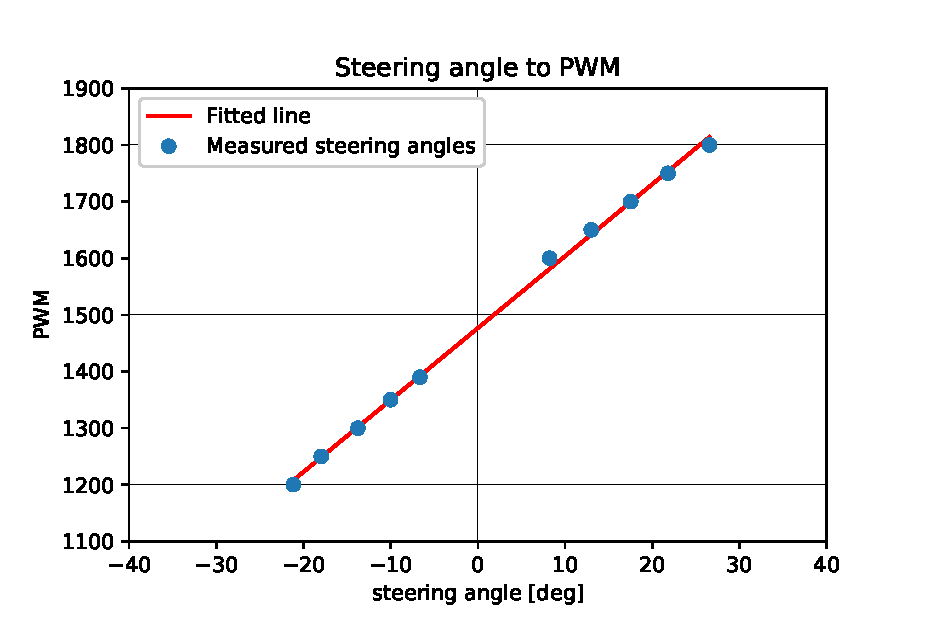
\includegraphics[width=\textwidth]{../img/steering_angle_to_pwm}
	\caption{The measurement shows the imperfections in the hardware construction. The vehicle is able to go around circles with smaller radii when it is turning left (positive steering angles) than when it is turning right (negative steering angles).}
	\label{fig:steering_angle_to_pwm}
\end{figure}

\paragraph{Servo Setting Time}

It takes non-trivial time for the steering servo to move from its previous position to a newly set position. The steering angle changes continuously as the servo adjusts and it affects the direction in which the vehicle travels in the meantime. In this experiment, we measure the setting time of the servo between different steering angles and based on the data, we will find a relationship between the distance between the servo position and the time it will take to set.

The position of the servo is set through a \gls{PWM} value between \SI{1200}{\micro\second} (rightmost position), \SI{1500}{\micro\second} (center position), and \SI{1800}{\micro\second} (leftmost position). In this procedure, the vehicle switches between a right position $r$ and a left position $l$ a hundred times while the vehicle is stationary and it is placed on a flat surface. The servo produces a noise during the whole setting period and is mostly quiet during the periods between adjustments.

We record the sound the servo makes through a microphone. The audio track is then edited using \textit{Audacity}\footnote{https://www.audacityteam.org/} to remove background noise and low frequency ``buzzing'' of the servo and to use the ``Sound Finder'' analysis tool to label periods of sound in the cleaned audio track (see Figure~\ref{fig:audacity}). The start and end times of the labeled intervals are then exported into a text file for further analysis.

We carried out this procedure for five pairs of \gls*{PWM} values: $(1800, 1200)$, $(1750, 1250)$, $(1700, 1300)$, $(1650, 1450)$, $(1600, 1400)$. Each of these pairs is symmetrical around the center position \SI{1500}{\micro\second} and the \textit{distance} between the two positions decreases from \SI{600}{\micro\second} to \SI{200}{\micro\second}. This might have biased the results and decrease the accuracy of our result.

\begin{figure}
	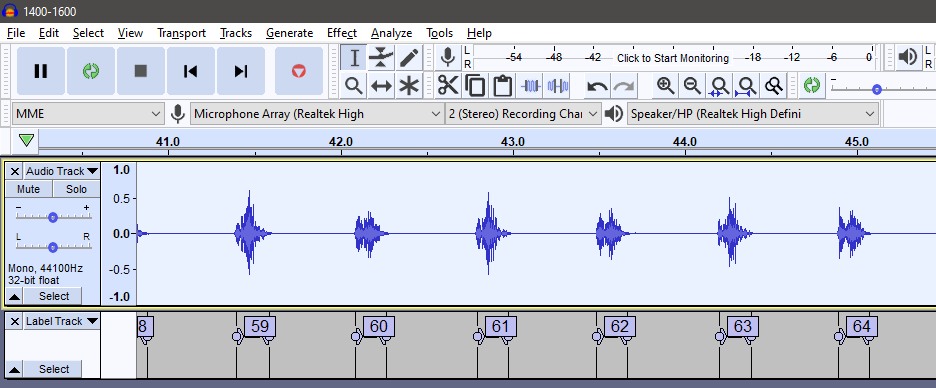
\includegraphics[width=\textwidth]{../img/servo_experiment_audacity}
	\protect\caption{The servo setting periods are clearly identifiable in an audio recording after background noise and low frequency sounds are removed. This figure shows the interface of the \textit{Audacity} tool used to analyze a recording of adjustments between the PWM signal of \SI{1400}{\micro\second} and \SI{1600}{\micro\second}.}
	\label{fig:audacity}
\end{figure}

We used the method of least squares to find a best fitting line in the form of $t=ad+b$, where $t$ is the setting time in seconds and $d$ is the distance between the \gls*{PWM} values. Based on the data we recorded, the relationship between the distance to the new servo position and the setting time is visualized in the Figure~\ref{fig:servo_linear_regression} and in the following equation:

\begin{equation}
\label{eq:servo_setting_time}
\begin{aligned}
t(d)&=0.000329\cdot d + 0.1174\\
t(\alpha,\beta)&=t(\abs{PWM(\alpha)-PWM(\beta)}),
\end{aligned}
\end{equation}

where $\alpha,\beta\in\left[\delta_{min}, \delta_{max}\right]$.

\begin{figure}
	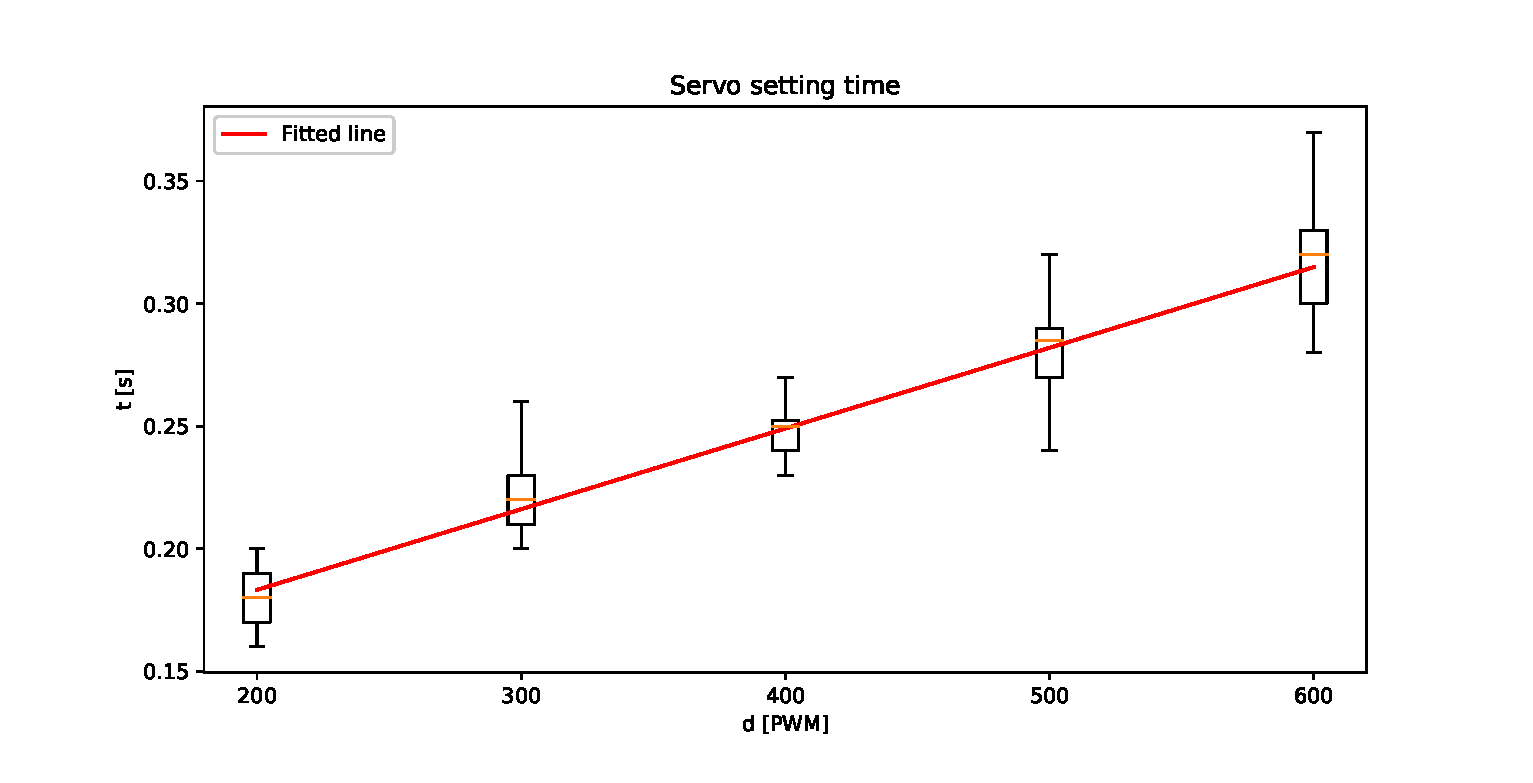
\includegraphics[width=\textwidth]{../img/servo_setting_time_linreg.eps}
	\caption{The setting time of the steering servo can be estimated with a linear function of the distance between the start and end PWM values.}
	\label{fig:servo_linear_regression}
\end{figure}

\paragraph{Steering Angle Model}

With the knowledge of how long it takes to adjust the steering angle of the front wheels, we can formulate the rate of change of the steering angle $\dot{\delta}$ in radians per second based on the current steering angle $\delta$ and target steering angle $\delta_t$:

\begin{equation}
\begin{aligned}
\Delta \delta&=\min\left\{\abs{\delta-\delta_t}, 2\pi-\abs{\delta-\delta_t}\right\}\\
\dot{\delta}&=\nicefrac{\sign{} \Delta \delta}{t(\delta, \delta_t)}.
\end{aligned}
\end{equation}

\subsubsection{DC Motor Model}

We need to be able to model the angular velocity of the motor shaft. The motor is directly connected to the wheels. Therefore, if we can predict the velocity at which the motor shaft rotates, we can predict how fast the wheels will turn. If the motor spins at angular velocity of $\omega$, then the angular velocity of the wheels $\omega_w$ will be equal to

\[
\omega_w = G\omega,
\]

where $G$ is a combined gear ratio of the gearbox and the differential. For a vehicle with multiple gears, this relationship would be a function of the selected gear. Because our experimental vehicle will have a single fixed gear, which is typical for electric cars, our gear ratio $G$ will be constant.

This, of course, does not give us all the information to determine the longitudinal velocity of the vehicle, because the wheels might skid when the friction forces between the tires and the road surface are exceeded.

Our goal is to create a model of the engine RPM as a function of the previous \gls{RPM} and the control inputs. We measured the RPM of the motor shaft using a Hall effect encoder while we were manually controlling the vehicle on dry asphalt at a temperature of around \SI{15}{\degreeCelsius}. We also recorded the throttle and steering angle inputs from the remote control. We use the collected data to identify the parameters of our model and to validate the accuracy of the model.

The torque of the motor depends directly on the speed at which its axle rotates. For a DC motor, the relationship can be approximated with a linear function which depends on two parameters: the maximum angular velocity $\omega_{max}$ and stall torque $T_{stall}$ as it is shown in Figure~\ref{fig:torque_rpm_curve}. The maximum angular velocity is measured with full throttle when there is no load on the motor and the stall torque is reached when the vehicle starts moving from standstill.

The throttle control input $\tau_t$ limits the amount of torque transferred to the wheels. The torque is counteracted by the load on the motor, e.g., friction or air resistance. While driving the experimental car manually, we learned that the steering angle $\delta$ of the front wheels is one of the most significant factors limiting the speed of the motor. When the car is at its maximum speed and the throttle is released, the car will travel a significant distance before it comes to a full stop. When the steering angle is large, the car stops almost immediately. The vehicle reaches a lower speed when it travels around a circle compared to going straight when full throttle is applied. The rate of change of angular velocity of a rigid body is equal to the total torque applied to the body divided by its moment of inertia.

We model the rate of change of the angular velocity of the motor with the following set of parametric equations, which are inspired by the mechanics of the motor:

\begin{equation}
\begin{aligned}
\label{eq:motor_model}
T_{max}&=\left(1 - \dfrac{\omega}{\omega_{max}}\right)x_1 \\
T_{drive}&=T_{max}\cdot \tau_t \\
T_{load}&=\omega^{x_2} \left(x_3 + x_4|\delta_t|\right)^{x_5} \\
\dot{\omega}&=\dfrac{T_{drive}-T_{load}}{x_6}.
\end{aligned}
\end{equation}

By integrating the $\dot{\omega}$ numerically over a time period $\Delta t$, we will obtain the change in the RPM of the vehicle. The parameters $x_i\in\mathbb{R}$ are obtained using a numerical optimization algorithm which minimizes mean squared error between the predicted RPM and RPM measured using the experimental vehicle. The parameter $x_1$ replaces $T_{stall}$ and $x_6$ replaces the moment of inertia of the power train. Nevertheless, the values assigned to these parameters by the optimization algorithm must not be interpreted as the values of these two properties.

An example prediction of our model with the fitted parameters as stated in Table~\ref{table:motor_model_params} is shown in Figure~\ref{fig:motor_rpm_model} for a time period of almost two minutes. The \gls*{RPM} shown in this figure is relative to the maximum \gls*{RPM} of the motor which we identified to be \SI{15500}{RPM}.

\begin{table}[h]
	\centering
	\begin{tabular}{l | l}
		$x_1$ & \num{7.33016701e+02} \\
		$x_2$ & \num{8.58626896e+02} \\
		$x_3$ & \num{7.40739969e-01} \\
		$x_4$ & \num{7.68248846e+01} \\
		$x_5$ & \num{2.05190302e+02} \\
		$x_6$ & \num{1.16584276e+00} \\
	\end{tabular}
	\caption{Fitted parameters of the DC motor model.}
	\label{table:motor_model_params}
\end{table}

We also tried training a neural network with three input neurons and one output neuron to predict $\dot{\omega}$ or $\omega$ directly. We experimented with supervised learning and with reinforcement learning using neuro-evolution (NEAT) but we were not able to obtain a neural network with better estimates of $\omega$ than the predictions from the model described in (\ref{eq:motor_model}).

\begin{figure}
	\centering
	
	\begin{tikzpicture}
	
	% the axes
	\draw[thick, ->] (-1,0)--(8,0) node[right]{$RPM$};
	\draw[thick, ->] (0,-1)--(0,6) node[above]{$torque$};
	
	\draw[ultra thick] (0, 4.5) node[left]{$T_{stall}$}--(7, 0)node[below]{$\omega_{max}$};
	
	\end{tikzpicture}
	
	\caption{Linear approximation of a DC motor torque curve. This linear model has two parameters: the maximum RPM without any load $\omega_{max}$ and stall torque $T_{stall}$.}
	\label{fig:torque_rpm_curve}
\end{figure}

\begin{figure}
	\centering
	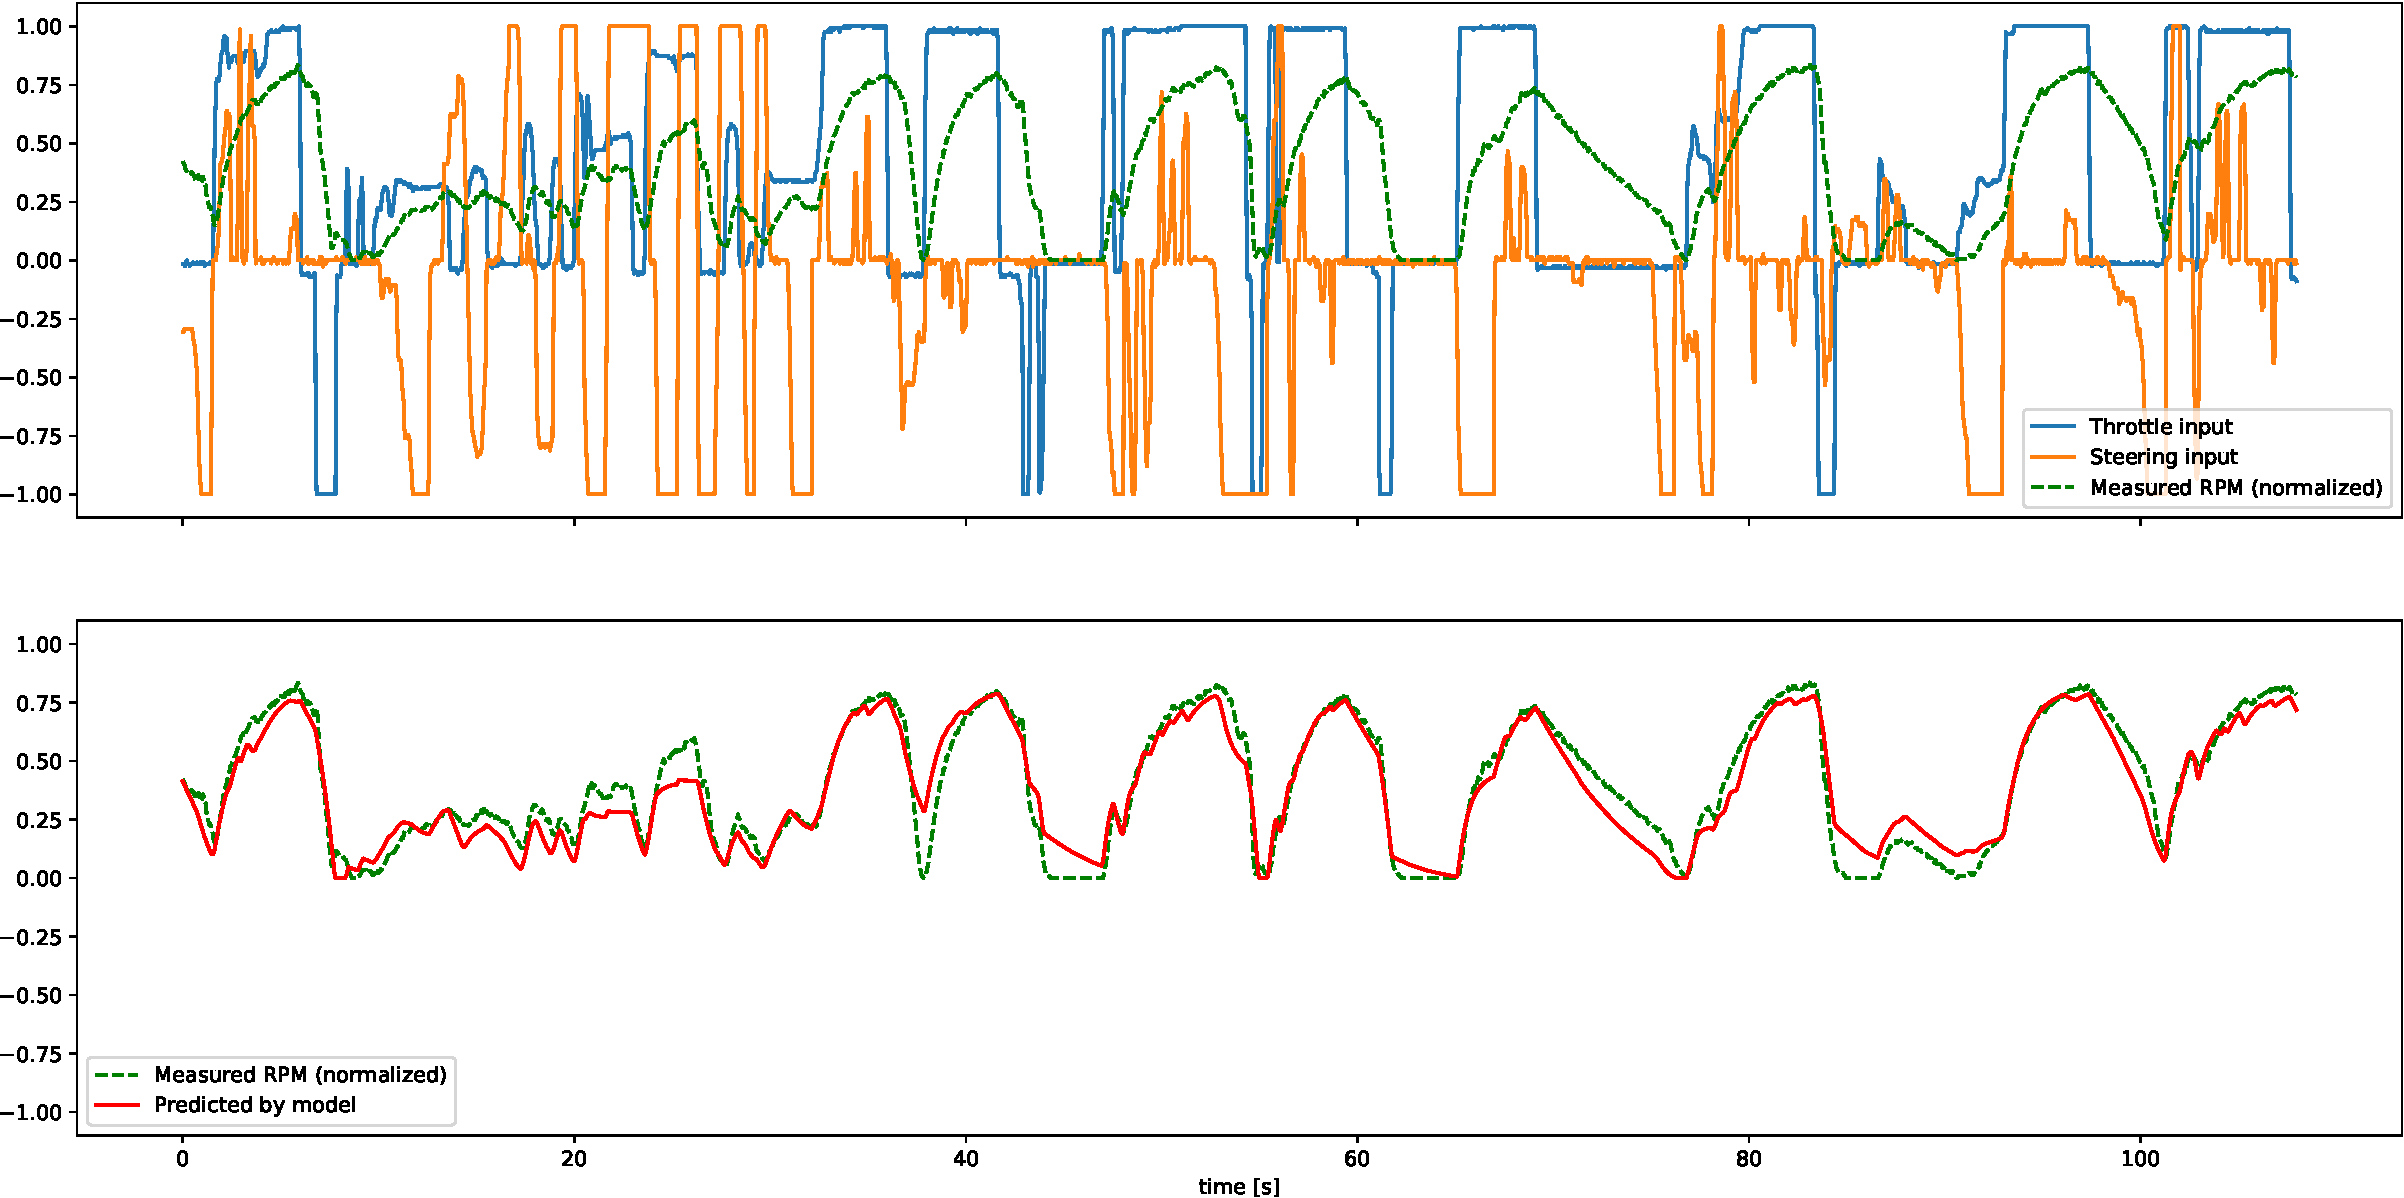
\includegraphics[width=\textwidth]{../img/fit_8000}
	\caption{The first chart shows the throttle and steering inputs as well as the measured RPM (normalized). The second chart compares the measured and predicted RPMs for the same time period using the fitted parameters of our model.}
	\label{fig:motor_rpm_model}
\end{figure}

\subsection{Kinematic Bicycle Model}

The name of the bicycle model, sometimes also referred to as one-track or single-track model in literature, comes from the fact, that we combine the effects of the two front wheels and the two rear wheels into a single virtual wheel located at the centers of the axles. Our kinematic model is based on a model described by Dr. Rajesh Rajamani \cite[Chapter~2]{rajamani} and it is visualized in Figure~\ref{fig:kinematic_bicycle}.

\begin{figure}[h!]
	\centering
	
	\begin{tikzpicture}[
	axis/.style={thin, densely dashed, gray},
	axle/.style={thick, gray},
	vec/.style={ultra thick, ->, >=latex}
	]
	
	% the axes
	\path[name path=AX] (-1,0)--(6,0);
	\draw[thin, ->] (-0.5,0)--(6,0) node[right]{$x$};
	\draw[thin, ->] (0,-0.5)--(0,4.5) node[above]{$y$};
	
	\def\lr{3}
	\def\lf{3}
	\def\L{\lr+\lf}
	\def\wW{0.55} % wheel width
	\def\wL{1.25} % wheel length
	\def\xoffset{2cm}
	\def\yoffset{1.5cm}
		
	\def\stateTheta{45} % heading angle of the vehicle
	\def\stateDelta{-35} % steering angle of the front wheels
	\def\stateBeta{-17.5} % steering angle of the front wheels
	
	% the rotated vehicle
	\begin{scope}[xshift=\xoffset, yshift=\yoffset]
	\begin{scope}[rotate=\stateTheta]
	
	% longitudinal axis
	\path[name path=AL] (-2.5, 0) -- (\L+2, 0);
	\draw[axis] (-2.2, 0) -- (\L+2, 0);
	
	% visualize theta
	\path[name intersections={of=AL and AX, by={X}}];
	\draw[rotate=-\stateTheta] (X)++(0.5,0) arc (0:\stateTheta:0.5) node[right, yshift=-0.5mm, xshift=1mm] {$\theta$}; % theta
	
	% axle coordinates
	\def\rearX{0}
	\def\centerX{\lr}
	\def\frontX{\L}
	
	\coordinate (front) at (\frontX, 0);
	\coordinate (cog) at (\lr, 0);
	\coordinate (rear) at (\rearX, 0);
	
	% visualize the wheelbase length
	\draw[axis] (rear) -- ++(0, 2);
	\draw[axis] (cog) -- ++(0, 2);
	\draw[axis] (front) -- ++(0, 2);
	\draw[<->, >=latex] ($ (rear) + (0, 1.5) $) -- node[above, xshift=-1.5mm, yshift=-1mm] {$l_r$} ($ (cog) + (0, 1.5) $);
	\draw[<->, >=latex] ($ (cog) + (0, 1.5) $) -- node[above, xshift=-1.5mm, yshift=-1mm] {$l_f$} ($ (front) + (0, 1.5) $);
	
	% connect the axles
	\draw[axle] (front) -- (rear);
	
	% wheels
	\draw[thick] (\rearX - \wL/2, -\wW/2) rectangle (\rearX + \wL/2, \wW/2); % rear wheel/tire
	\draw[thick, rotate around={\stateDelta:(\frontX, 0)}] (\frontX - \wL/2, -\wW/2) rectangle (\frontX + \wL/2, \wW/2); % front wheel/tire
	
	% center of gravity
	\filldraw[thick] (cog) circle (2pt) node[below, xshift=4mm, yshift=-1mm] {$(x, y)$};

	% visualize delta
	\draw[axis, rotate around={\stateDelta:(front)}] (front) -- ++(2, 0);
	\draw (front)++(1.2,0) arc (0:\stateDelta:1.2) node[right, yshift=5mm] {$\delta$}; % delta
	
	% visualize beta/velocity
	\draw[vec, rotate around={\stateBeta:(cog)}] (cog) -- node[below, xshift=3mm] {$v$} ++(1.5, 0);
	\draw (cog)++(1,0) arc (0:\stateBeta:1) node[right, yshift=4.25mm, xshift=1mm] {$\beta$}; % beta
	
	\end{scope}
	\end{scope}
	
	\end{tikzpicture}
	
	\caption{The two front and two rear wheels are merged into a single wheel at the center of each axle for simplification. The $(x,y)$ position of the center of gravity moves at the speed $v$ in the direction $\theta+\beta$ in the global reference frame.}
	\label{fig:kinematic_bicycle}
\end{figure}

We assume that the wheels are rolling in the same direction in which they are pointing. When the front wheels are turned to a steering angle $\delta\neq 0$, our vehicle will be going around a circle with a constant radius. We will also assume that the wheels are rolling against the road surface and that the vehicle never loses traction.

These simplifications will cause our model to be imprecise during high speed cornering, when the car can start ``drifting'' when the wheels lose grip and the vehicle will start moving sideways.

Since the motor is directly connected to the wheels and we assume that the wheels are rolling perfectly against the surface, the speed of the vehicle is directly proportional to the engine angular velocity:

\begin{equation*}
v=\omega_w r,
\end{equation*}

where $r$ is the radius of the wheels and $\omega_w$ is the angular velocity of the wheels.

Based on the no-slip condition, all the wheels are moving at the same speed $v$ but in a different direction. The rear virtual wheel is moving in the heading direction of the vehicle $\theta$ and the front wheels in the direction they are pointing $\theta + \delta$. Therefore, the center of gravity will not move in the direction of the orientation of the vehicle, but it will be slightly offset by the steering angle $\delta$. From the geometry of the vehicle, we can determine the direction, in which the center of gravity will move:

\begin{equation*}
	\beta=\arctan\left(\dfrac{l_r}{l_r+l_f}\tan\delta\right).
\end{equation*}

The linear and rotational velocity of the body of the vehicle in the global reference frame is described by these equations:

\begin{equation*}
\begin{aligned}
\dot{x}&=v\cos\left(\theta + \beta\right) \\
\dot{y}&=v\sin\left(\theta + \beta\right) \\
\dot{\theta}&=\dfrac{v\cos\beta\tan\delta}{l_r + l_f}.
\end{aligned}
\end{equation*}

The kinematic model does not require any extra state variables on top of the configuration and the state variables of the actuators. The final state space $X$ would therefore have five continuous dimensions:

\begin{equation*}
	X=\left\{\left(x,y,\theta,\delta,\omega\right)\mid x,y,\omega\in\mathbb{R}, \theta,\delta\in\left[0, 2\pi\right)\right\}.
\end{equation*}

\subsection{Dynamic Bicycle Model}

Forces are the cause of linear and angular acceleration of every rigid body. The dynamic bicycle model models the forces between the tires of the vehicle and the road surface and describes the resulting accelerations. To describe the translation and rotation of the vehicle on a two dimensional plane, we need to know the values of two forces: the longitudinal forces $F_x$, which cause the motion forward or backward, and lateral forces $F_y$, which allow the vehicle to turn and which cause rotation of the vehicle. An overview of all of the forces and other important variables is shown in Figure~\ref{fig:dynamic_bicycle}.

If we knew the longitudinal forces of the wheels $F_{xr}$ and $F_{xf}$, we could determine the total traction force acting at the center of gravity of the vehicle and the subsequent acceleration $\dot{v}$ of the vehicle:

\begin{equation*}
\begin{aligned}
F_{traction}&=F_{xr}+F_{xf}\cos\delta-F_{yf}\sin\delta \\
\dot{v}&=\dfrac{1}{m}\left(F_{traction}-F_{load}\right).
\end{aligned}
\end{equation*}

where $m\in\mathbb{R}_+$ is the mass of the vehicle and $F_{load}$ is a longitudinal load force on the vehicle, consisting of an aerodynamic drag force and rolling resistance.

The vehicle moves in the direction of the slip angle $\beta$ and it rotates around its $z$ axis at the angular velocity $\dot{\theta}$. With the knowledge of the lateral forces $F_{yf}$ and $F_{yr}$ we can model the behavior of these state variables:

\begin{equation*}
\begin{aligned}
\dot{\beta}&=\dfrac{1}{mv}\left(F_{yf}\cos\delta+F_{yr}\right)-\dot{\theta} \\
\ddot{\theta}&=\dfrac{1}{I_z}\left(l_f \left(F_{yf}\cos\delta - F_{xf}\sin\delta \right) - l_r F_{yr}\right),
\end{aligned}
\end{equation*}

where $I_z$ is the angular momentum of the vehicle around the $z$ axis which is the rotational equivalent of mass.

The change of the coordinates center of gravity of the vehicle in the two dimensional plane is then calculated the same way as we did in the kinematic model:

\begin{equation*}
\begin{aligned}
\dot{x}&=v\cos\left(\theta + \beta\right) \\
\dot{y}&=v\sin\left(\theta + \beta\right).
\end{aligned}
\end{equation*}

\begin{figure}[h!]
	\centering
	
	\begin{tikzpicture}[
	axis/.style={thin, densely dashed, gray},
	axle/.style={thick, gray},
	vec/.style={ultra thick, ->, >=latex}
	]
	
	% the axes
	\path[name path=AX] (-1,0)--(6,0);
	\draw[thin, ->] (-0.5,0)--(6,0) node[right]{$x$};
	\draw[thin, ->] (0,-0.5)--(0,4.5) node[above]{$y$};
	
	\def\lr{3}
	\def\lf{3}
	\def\L{\lr+\lf}
	\def\wW{0.55} % wheel width
	\def\wL{1.25} % wheel length
	\def\xoffset{2.0cm}
	\def\yoffset{1.5cm}
	
	\def\stateTheta{45} % heading angle of the vehicle
	\def\stateDelta{-35} % steering angle of the front wheels
	\def\stateBeta{-17.5} % steering angle of the front wheels
	
	% the rotated vehicle
	\begin{scope}[xshift=\xoffset, yshift=\yoffset]
	\begin{scope}[rotate=\stateTheta]
	
	% longitudinal axis
	\path[name path=AL] (-2.5, 0) -- (\L+2, 0);
	\draw[axis] (-2.2, 0) -- (\L+2, 0);
	
	% visualize theta
	\path[name intersections={of=AL and AX, by={X}}];
	\draw[rotate=-\stateTheta] (X)++(0.5,0) arc (0:\stateTheta:0.5) node[right, yshift=-0.5mm, xshift=1mm] {$\theta$}; % theta
	
	% axle coordinates
	\def\rearX{0}
	\def\centerX{\lr}
	\def\frontX{\L}
	
	\coordinate (front) at (\frontX, 0);
	\coordinate (cog) at (\lr, 0);6
	\coordinate (rear) at (\rearX, 0);
	
	% visualize the wheelbase length
	\draw[axis] (rear) -- ++(0, 2);
	\draw[axis] (cog) -- ++(0, 2);
	\draw[axis] (front) -- ++(0, 2);
	\draw[<->, >=latex] ($ (rear) + (0, 1.5) $) -- node[above, xshift=-1.5mm, yshift=-1mm] {$l_r$} ($ (cog) + (0, 1.5) $);
	\draw[<->, >=latex] ($ (cog) + (0, 1.5) $) -- node[above, xshift=-1.5mm, yshift=-1mm] {$l_f$} ($ (front) + (0, 1.5) $);

	% connect the axles
	\draw[axle] (front) -- (rear);
	
	% wheels
	\draw[thick] (\rearX - \wL/2, -\wW/2) rectangle (\rearX + \wL/2, \wW/2); % rear wheel/tire
	\draw[thick, rotate around={\stateDelta:(\frontX, 0)}] (\frontX - \wL/2, -\wW/2) rectangle (\frontX + \wL/2, \wW/2); % front wheel/tire

	% center of gravity
	\filldraw[thick] (cog) circle (2pt) node[below, xshift=4mm, yshift=-1mm] {$(x, y)$};
	
	% visualize delta
	\draw (front)++(1.2,0) arc (0:\stateDelta:1.2) node[right, yshift=5mm] {$\delta$}; % delta
	
	% visualize beta/velocity
	\draw[vec, rotate around={\stateBeta:(cog)}] (cog) -- node[below, xshift=3mm] {$v$} ++(1.5, 0);
	\draw (cog)++(1,0) arc (0:\stateBeta:1) node[right, yshift=4.25mm, xshift=1mm] {$\beta$}; % beta
	
	% forces	
	\draw[vec] (rear) -- ++(0, -1) node[right, xshift=-0.1mm, yshift=0.5mm] {$F_{yr}$};
	\draw[vec, rotate around={\stateDelta:(\frontX, 0)}] (front) -- ++(0, -1) node[right] {$F_{yf}$};
	\draw[vec] (rear) -- ++(2, 0) node[below, xshift=-1mm, yshift=-4mm] {$F_{xr}$};
	\draw[vec, rotate around={\stateDelta:(\frontX, 0)}] (front) -- ++(2, 0) node[below, xshift=1.75mm] {$F_{xf}$};
	\draw[vec] (cog) -- ++(2.25, 0) node[left, xshift=-8mm, yshift=-4.5mm] {$F_{traction}$};
	\draw[vec] (cog) -- ++(-0.75, 0) node[above, xshift=-1.5mm, yshift=2mm] {$F_{load}$};

	\end{scope}
	\end{scope}
	
	\end{tikzpicture}
	
	\caption{The dynamic model calculates the acceleration and the yaw rate based on the forces which act on the body of the vehicle. The configuration $(x, y, \theta)$ represents the position of the center of gravity of the vehicle and the heading angle in the global reference frame.}
	\label{fig:dynamic_bicycle}
\end{figure}

\subsubsection{Tire Model}

A tire is an interface between the road and the vehicle. The engine produces torque which is transferred to the wheels through the drive train and this torque is translated into a force at the contact patch between the tires and the road. This force is what puts the vehicle into motion, and what allows the vehicle to turn by changing the steering angle. 

There are several mathematical tire models, such as Brush, Fiala, Dugoff, or Pacejka models \cite{rajamani, pacejka}, which describe how to calculate the tire forces $F_x$ and $F_y$. The problem with these models is that they require a knowledge of many parameters, which must be obtained through experimental measurements of the properties of the actual vehicle.

This turned out to be a problem for us. Even though some students performed identification of the Pacejka magic formula parameters for a similar RC car model \cite{rc_identification, rc_identification_2}, we were not able to perform the measurements and obtain good quality tire model for our custom experimental vehicle. We are therefore unable to utilize the properties of the dynamic bicycle model to describe our experimental vehicle.

\subsection{Discussion}

We are now able to describe the movement of the vehicle based on the throttle level and target steering angle inputs. The models of the steering servo and of the DC motor were obtained empirically by measuring the responses of the hardware to the control inputs. Especially the model of the DC motor is interesting, because it predicts the RPM of the motor not only based on the throttle level, but also on the angle of the wheels. This reflects how the vehicle loses its kinetic energy during cornering.

Due to our inability to precisely measure the parameters of tire models, we have to use a simplified kinematic model with a no-slip assumption for our experiments. The planner might be too optimistic find trajectories which are too aggressive and the vehicle will not be able to follow them precisely. We would be improve the trajectories found by our planner if we obtained the dynamic model in the future or if we were able to try our algorithm on a different vehicle for which we knew the parameters of a tire model. On the other hand, the dynamic model has two additional dimensions of the state space (the slip angle $\beta$ and the yaw rate $\dot{\theta}$), which will make the computation task harder.
